\chapter{QR分解与Householder变换}

\section{Triangular Matrices}

\begin{definition}[Lower Triangular Matrices]
    矩阵 $  {A} \in \mathfrak{R}^{n \times n} $ 为\term{下三角(Lower Triangular)矩阵}, $ A_{i j}=0, j>i $ .

    \begin{equation} A=\left[\begin{array}{ccccc}A_{11} & 0 & \cdots & 0 & 0 \\ A_{21} & A_{22} & \cdots & 0 & 0 \\ \vdots & \vdots & \ddots & \vdots & \vdots \\ A_{n-1,1} & A_{n-1,2} & \cdots & A_{n-1, n-1} & 0 \\ A_{n 1} & A_{n 2} & \cdots & A_{n, n-1} & A_{n n}\end{array}\right] \end{equation}
\end{definition}

\begin{definition}[Upper Triangular Matrices]
    $ A^{T} $ 为\term{上三角(Upper Triangular)矩阵}.

    \begin{equation} A=\left[\begin{array}{ccccc}A_{11} & A_{12} & \cdots & A_{1, n-1} & A_{1, n} \\ 0 & A_{22} & \cdots & A_{2, n-1} & A_{2, n} \\ \vdots & \vdots & \ddots & \vdots & \vdots \\ 0 & 0 & \cdots & A_{n-1, n-1} & A_{n-1, n} \\ 0 & 0 & \cdots & 0 & A_{n n}\end{array}\right] \end{equation}
\end{definition}

\begin{definition}[单位上三角矩阵,单位下三角矩阵]
    对角元素 $ a_{i i} $ 都等于 1的上(下)三角矩阵。
\end{definition}

\subsection{高斯消元法}

\begin{problem}
    当 $ A $ 是具有非零对角元素的下三角矩阵时,解 $ A x=b $ .
\end{problem}

使用\term{前向回代(Forward Substitution)}算法求解。

\begin{theorem}[前向回代时间复杂度]
    \label{complexity:forward-substitution}
    $ 1+3+5+\ldots+(2  {n}-1)= {n}^{2} $ flops
\end{theorem}

\begin{algorithm}[htbp]
    \caption{Forward Substitution}
    \KwIn{$A \in \mathfrak{R}^{n \times n} (A是下三角矩阵), b \in \mathfrak{R}^{n \times 1}$}
    \KwOut{$x \in \mathfrak{R}^{n \times 1}$}
    $ x_{1}= \dfrac{b_{1} }{A_{11} }  $\;
$ x_{2}=\dfrac{b_{2}-A_{21} x_{1}}{A_{22}}$\;
$  x_{3} =\dfrac{b_{3}-A_{31} x_{1}-A_{32} x_{2}}{A_{33}} $ \;
    $\cdots$  \;
    $x_{n} =
    \dfrac{b_{n}-A_{n 1} x_{1}-A_{n 2} x_{2}-\cdots-A_{n, n-1} x_{n-1}}{A_{n n}} $\;
\end{algorithm}

\begin{problem}
    当$A$是具有非零对角元素的上三角矩阵, 解 $  {A} x= {b} $ .
\end{problem}

使用\term{后向回代(Back Substitution)}算法来求解。

\begin{algorithm}[htbp]
    \caption{Backward Substitution}
    \KwIn{$A \in \mathfrak{R}^{n \times n} (A是上三角矩阵), b \in \mathfrak{R}^{n \times 1}$}
    \KwOut{$x \in \mathfrak{R}^{n \times 1}$}
    $ x_{n}= \dfrac{b_{n}}{A_{n n}} $\;
    $ x_{n-1}= \dfrac{b_{n-1}-A_{n-1, n} x_{n}}{A_{n-1, n-1}} $ \;
    $ x_{n-2}= \dfrac{b_{n-2}-A_{n-2, n-1} x_{n-1}-A_{n-2, n} x_{n}}{ A_{n-2, n-2}} $\;
    $\cdots$\;
    $ x_{1}=\dfrac{b_{1}-A_{12} x_{2}-A_{13} x_{3}-\cdots-A_{1 n} x_{n}}{A_{11}}  $\;
\end{algorithm}

\begin{theorem}[后向回代时间复杂度]
    $ 1+3+\ldots+2  {n}-1= {n}^{2} $ flops
\label{complexity:Backward-Substitution}
\end{theorem}



\subsection{The Inverses of Triangular Matrices}

\begin{theorem}
    对角元素非零的三角矩阵$A$是非奇异的,即:
\begin{equation}
A x=0 \quad \Rightarrow \quad x=0
\end{equation}
\end{theorem}

\begin{theorem}[高斯消元法]
    $A$的逆可以通过逐列解方程$AX=I$来计算得到

    \begin{equation} A\left[\begin{array}{llll}x_{1} & x_{2} & \cdots & x_{n}\end{array}\right]=\left[\begin{array}{llll}e_{1} & e_{2} & \cdots & e_{n}\end{array}\right] \end{equation}
\end{theorem}

\begin{theorem}
    下三角矩阵的逆是下三角矩阵,上三角矩阵的逆是上三角矩阵。
\end{theorem}

\begin{theorem}[计算上/下三角矩阵 $  {A} \in \mathfrak{R}^{n \times n} $ 逆的复杂度]
    \label{complexity:inverse-of-triangular}

\begin{equation} n^{2}+(n-1)^{2}+\cdots+1 \approx \frac{1}{3} n^{3}\text{ flops }\end{equation} 
\end{theorem}



\section{QR Factorization}



如果矩阵 $ A \in \mathfrak{R}^{m \times n} $ 的列向量线性无关,则可以将其分解为

\begin{theorem}[QR Factorization]
    
    \begin{equation}\begin{aligned} A_{n  \times n}&=\left[\begin{array}{llll}a_{1} & a_{2} & \cdots & a_{n}\end{array}\right]\\
        &=\left[\begin{array}{llll}q_{1} & q_{2} & \cdots & q_{n}\end{array}\right]\left[\begin{array}{cccc}R_{11} & R_{12} & \cdots & R_{1 n} \\ 0 & R_{22} & \cdots & R_{2 n} \\ \vdots & \vdots & \ddots & \vdots \\ 0 & 0 & \cdots & R_{n n}\end{array}\right]\\
        &=Q_{n  \times n}R_{n  \times  n}
        \end{aligned}\end{equation}

向量 $ q_{1}, \ldots, q_{n} \in \mathfrak{R}^{m} $ 是标准正交向量:
\begin{equation}
\left\|q_{i}\right\|_{2}=1, \quad q_{i}^{T} q_{j}=0, \text { if } \quad i \neq j
\end{equation}

对角元素 $ R_{i i} $ 是非零的。若 $ R_{i i}<0 $, 改变 $ R_{i i}, \cdots, R_{i n} $ 和向量 $ q_{i} $ 的符号。大多数定义要求 $ R_{i i}>0 $,使得$Q$和$R$是唯一的。
\end{theorem}

\begin{remark}
    下面各节均假定矩阵 $ A \in \mathfrak{R}^{m \times n} $ 的列向量线性无关。
\end{remark}

\begin{corollary}
    $ Q \in \mathfrak{R}^{m \times n} $ 具有标准正交列 $ \left(Q^{T} Q=I\right) $.
\end{corollary}

\begin{corollary}
    如果 $ A $ 是方阵 $ ( {m}= {n}) $, 则 $ Q $ 是正交的 $ \left(Q^{T} Q=Q Q^{T}=I\right) $.
\end{corollary}

\begin{corollary}
    $ R \in \mathfrak{R}^{n \times n} $ 的上三角矩阵。
\end{corollary}

\begin{corollary}
     $ R $ 是非奇异的(对角元素是非零的).
\end{corollary}

\begin{corollary}
    \begin{equation} R=Q^{-1} A \Rightarrow R=Q^{T} A \end{equation}
\end{corollary}

QR分解可通过Gram-Schmidit正交化法(参见\ref{Chap:Gram-Schmidt Algorithm})、Householder变换等进行。

More generally, we can factor a complex $ m \times n $ matrix $ A $, with $ m \geq n $, as the product of an $ m \times m $ unitary matrix $ Q $ and an $ m \times n $ upper triangular matrix $ R $. As the bottom $ (m-n) $ rows of an $ m \times n $ upper triangular matrix consist entirely of zeroes, it is often useful to partition $ R $, or both $ R $ and $ Q $ :
\begin{equation}
A=Q R=Q\left[\begin{array}{c}
R_{1} \\
0
\end{array}\right]=\left[\begin{array}{ll}
Q_{1} & Q_{2}
\end{array}\right]\left[\begin{array}{c}
R_{1} \\
0
\end{array}\right]=Q_{1} R_{1}
\end{equation}
where $ R_{1} $ is an $ n \times n $ upper triangular matrix, 0 is an $ (m-n) \times n $ zero matrix, $ Q_{1} $ is $ m \times n, Q_{2} $ is $ m \times(m-n) $, and $ Q_{1} $ and $ Q_{2} $ both have orthogonal columns.

Golub \& Van Loan (1996) call $ Q_{1} R_{1} $ the \term{thin $ Q R $ factorization of $ A $}; Trefethen and Bau call this the \term{reduced QR factorization}.   If $ A $ is of full rank $ n $ and we require that the diagonal elements of $ R_{1} $ are positive then $ R_{1} $ and $ Q_{1} $ are unique, but in general $ Q_{2} $ is not. $ R_{1} $ is then equal to the upper triangular factor of the Cholesky decomposition of $ A^{*} A$ ($=A^{\top} A $ if $ A $ is real).


\begin{algorithm}[htbp]
    \caption{QR Decomposition Using Gram-Schmidt Algorithm}
    
    设矩阵 $ A $ 的列向量依次为 $ a_{1}, a_{2}, \cdots, a_{n} $ ,由于 $ A $ 为非奇异矩阵, 则列向量线性无关\;
    对列向量 $ a_{1}, a_{2}, \ldots, a_{n} $ 按照Gram-Schmidt方法进行正交化,然后单位化\;
    单位化得到的标准正交向量 $ q_{1}, q_{2}, \ldots, q_{n} $, 即得到标准正交矩阵$Q$\;
    根据 $ R=Q^{-1} A \Rightarrow R=Q^{T} A $, 得到上三角矩阵$R$\;
    $ Q R $ 分解 $ A=Q R $\;
\end{algorithm}

\begin{example}
    矩阵$A$的QR分解过程

    \begin{equation} A=\left[\begin{array}{ccc}1 & 1 & 0 \\ 1 & -1 & 1 \\ 0 & 0 & 2\end{array}\right] \end{equation}

    令 $ a_{1}=(1,1,0)^{T}, a_{2}=(1,-1,0)^{T}, a_{3}=(0,1,2)^{T} $, 由Gram-Schmidt方法正交单位化后, 得到 $ q_{1}=\left(\frac{1}{\sqrt{2}}, \frac{1}{\sqrt{2}}, 0\right)^{T}, q_{2}=\left(\frac{1}{\sqrt{2}},-\frac{1}{\sqrt{2}}, 0\right)^{T}, q_{3}=(0,0,1)^{T} $ .

    所以 $ a_{1}=\sqrt{2} q_{1}, \quad a_{2}=\sqrt{2} q_{2}, \quad a_{3}=\frac{1}{\sqrt{2}} q_{1}-\frac{1}{\sqrt{2}} q_{2}+2 q_{3} $ .

    \begin{equation} A=Q R=\left[\begin{array}{ccc}\frac{1}{\sqrt{2}} & \frac{1}{\sqrt{2}} & 0 \\ \frac{1}{\sqrt{2}} & -\frac{1}{\sqrt{2}} & 0 \\ 0 & 0 & 1\end{array}\right]\left[\begin{array}{ccc}\sqrt{2} & 0 & \frac{1}{\sqrt{2}} \\ 0 & \sqrt{2} & -\frac{1}{\sqrt{2}} \\ 0 & 0 & 2\end{array}\right] \end{equation}

\end{example}

\begin{example}
    \begin{equation}
\begin{aligned}
\left[\begin{array}{rrr}
-1 & -1 & 1 \\
1 & 3 & 3 \\
-1 & -1 & 5 \\
1 & 3 & 7
\end{array}\right] &=\left[\begin{array}{rrr}
-1 / 2 & 1 / 2 & -1 / 2 \\
1 / 2 & 1 / 2 & -1 / 2 \\
-1 / 2 & 1 / 2 & 1 / 2 \\
1 / 2 & 1 / 2 & 1 / 2
\end{array}\right]\left[\begin{array}{rrr}
2 & 4 & 2 \\
0 & 2 & 8 \\
0 & 0 & 4
\end{array}\right] \\
&=\left[\begin{array}{lll}
q_{1} & q_{2} & q_{3}
\end{array}\right]\left[\begin{array}{ccc}
R_{11} & R_{12} & R_{13} \\
0 & R_{22} & R_{23} \\
0 & 0 & R_{33}
\end{array}\right] \\
&=Q R
\end{aligned}
\end{equation}
\end{example}

\subsection[QR分解的存在唯一性]{QR分解的存在唯一性\footnote{Reference: \href{http://math.ecnu.edu.cn/~jypan/Teaching/SciComp/}{SciComp}, \href{https://www.math.purdue.edu/~kkloste/cs515fa14/qr-uniqueness.pdf}{Kyle Kloster's Website}}}

可以证明,QR分解具有唯一性。


\begin{theorem}[列满秩矩阵$A$的 QR 分解的存在唯一性]

    设 $A \in \mathbb{C}^{m \times n}(m \geq n)$. 则存在一个单位列正交矩阵 $Q \in \mathbb{C}^{m \times n}$ (即 $Q^{H} Q=$ $\left.I_{n \times n}\right)$ 和一个上三角矩阵 $R \in \mathbb{C}^{n \times n}$, 使得
\begin{equation}
A=Q R
\end{equation}
若 $A$ 列满秩, 则存在一个具有正对角线元素的上三角矩阵 $R$ 使得上式成立, 且此时 $Q R$ 分解唯一, 即 $Q$ 和 $R$ 都唯一。
\end{theorem}

\begin{proof}
    存在性: 
    
    由于 $A$ 列满秩, 由 Gram-Schmidt 正交化过程可知, 存在上三角矩阵 $R=\left[r_{i j}\right]_{n \times n}$ 满足 $r_{j j}>0$, 使得 $A=Q R$, 其中 $Q$ 单位列正交。

    唯一性: 
    
    假设 $A$ 存在 QR 分解
\begin{equation}
A=Q_{1} R_{1}=Q_{2} R_{2}
\end{equation}

其中 $Q_{1}, Q_{2} \in \mathbb{C}^{m \times n}$ 单位列正交, $R_{1}, R_{2} \in \mathbb{C}^{n \times n}$ 为具有正对角元素的上三角矩阵。 则有

\begin{equation}
    \label{eqn: q1-q2-r}
    Q_{1}=Q_{2} R_{2} R_{1}^{-1}
\end{equation}


由于 $R_{1}, R_{2}$ 均为上三角矩阵, 所以 $R_{2} R_{1}^{-1}$ 也是上三角矩阵, 且其对角线元素为 $\frac{R_{2_{i,i}}}{R_{1_{i,i}}}$, $i=1,2, \ldots, n$. 由 \cref{eqn: q1-q2-r} 可得

\begin{equation}
1=\left\|Q_{1}\right\|_{2}=\left\|Q_{2} R_{2} R_{1}^{-1}\right\|_{2}=\left\|R_{2} R_{1}^{-1}\right\|_{2}
\end{equation}

所以
\begin{equation}
\frac{R_{2_{i,i}}}{R_{1_{i,i}}} \leq 1, \quad i=1,2, \ldots, n
\end{equation}
同理可证$\frac{R_{2_{i,i}}}{R_{1_{i,i}}} \leq 1$. 所以
\begin{equation}
\frac{R_{2_{i,i}}}{R_{1_{i,i}}}, \quad i=1,2, \ldots, n
\end{equation}
又 $\left\|Q_{1}\right\|_{F}^{2}=\operatorname{tr}\left(Q_{1}^{T} Q_{1}\right)=n$, 所以由 \cref{eqn: q1-q2-r} 可知
\begin{equation}
\left\|R_{2} R_{1}^{-1}\right\|_{F}^{2}=\left\|Q_{2} R_{2} R_{1}^{-1}\right\|_{F}^{2}=\left\|Q_{1}\right\|_{F}^{2}=n
\end{equation}
由于 $R_{2} R_{1}^{-1}$ 的对角线元素都是 1 , 所以 $R_{2} R_{1}^{-1}$ 只能是单位矩阵, 即 $R_{2}=R_{1}$. 因此 $Q_{2}=A R_{2}^{-1}=$ $A R_{1}^{-1}=Q_{1}$, 即 $A$ 的 $ {QR}$ 分解是唯一的。

\end{proof}

% \begin{theorem}[$m=n $矩阵$A$进行QR分解的唯一性]
%     If $ \boldsymbol{A}=\boldsymbol{Q}_{1} \boldsymbol{R}_{1}=\boldsymbol{Q}_{2} \boldsymbol{R}_{2} $ are two QR decompositions of full rank, square $ A $, then
% \begin{equation}
% \begin{array}{l}
% \boldsymbol{Q}_{2}=\boldsymbol{Q}_{1} \boldsymbol{S} \\
% \boldsymbol{R}_{2}=\boldsymbol{S} \boldsymbol{R}_{1}
% \end{array}
% \end{equation}
% for some square diagonal $ \boldsymbol{S} $ with entries $ \pm 1 $. 

% If we require the diagonal entries of $ \boldsymbol{R} $ to be positive, then the decomposition is unique.
% \end{theorem}

% \begin{theorem}[$m<n $矩阵$A$进行QR分解的唯一性]
    
%     If \begin{equation}\boldsymbol{A}=\boldsymbol{Q}_{1}\left[\begin{array}{ll}\boldsymbol{R}_{1} & \boldsymbol{N}_{1}\end{array}\right]=\boldsymbol{Q}_{2}\left[\begin{array}{ll}\boldsymbol{R}_{2} & \boldsymbol{N}_{2}\end{array}\right]\end{equation} are two QR decompositions of a full rank, $m \times n$ matrix $\boldsymbol{A}$ with $m<n$, then

    
% \begin{equation}
% \boldsymbol{Q}_{2}=\boldsymbol{Q}_{1} \boldsymbol{S}, \quad \boldsymbol{R}_{2}=\boldsymbol{S R}_{1}, \quad \text { and } \quad \boldsymbol{N}_{2}=\boldsymbol{S} \boldsymbol{N}_{1}
% \end{equation}
% for square diagonal $S$ with entries $\pm 1$. 

% If we require the diagonal entries of $\boldsymbol{R}$ to be positive, then the decomposition is unique.

% \end{theorem}

% \begin{proof}
%     Let $\boldsymbol{Q}_{1}\left[\begin{array}{ll}\boldsymbol{R}_{1} & \boldsymbol{N}_{1}\end{array}\right]=\boldsymbol{Q}_{2}\left[\begin{array}{ll}\boldsymbol{R}_{2} & \boldsymbol{N}_{2}\end{array}\right]$ with $\boldsymbol{Q}_{i}$ being $m \times m$ and orthogonal, $\boldsymbol{R}_{i}$ being $m \times m$ and upper triangular, and $\boldsymbol{N}_{i}$ being an arbitrary $m \times(n-m)$ matrix. 
    
%     Then multiplying through yields $\boldsymbol{Q}_{1} \boldsymbol{R}_{1}=\boldsymbol{Q}_{2} \boldsymbol{R}_{2}$, two $ {QR}$ decompositions of a full rank, $m \times m$ matrix. 
    
%     Using the theorem above, we get that $\boldsymbol{Q}_{2}=\boldsymbol{Q}_{1} \boldsymbol{S}$ and $\boldsymbol{R}_{2}=\boldsymbol{S} \boldsymbol{R}_{1}$ for a diagonal matrix $\boldsymbol{S}$ with entries $\pm 1$. 
    
%     Looking at the right-most partition of the original product yields $\boldsymbol{Q}_{1} \boldsymbol{N}_{1}=\boldsymbol{Q}_{2} \boldsymbol{N}_{2}$. But we've shown $\boldsymbol{Q}_{2}=\boldsymbol{Q}_{1} \boldsymbol{S}$, so now we have $\boldsymbol{Q}_{1} \boldsymbol{N}_{1}=\boldsymbol{Q}_{1} \boldsymbol{S} \boldsymbol{N}_{2}$. 
    
%     Left-multiplying by $\boldsymbol{Q}_{1}^{T}$ and then by $\boldsymbol{S}$ then proves $\boldsymbol{N}_{2}=\boldsymbol{S} \boldsymbol{N}_{1}$, completing the theorem.
% \end{proof}

% \begin{theorem}[$m>n $矩阵$A$进行QR分解的唯一性]

%     If $\boldsymbol{A}=\left[\begin{array}{ll}\boldsymbol{Q}_{1} & \boldsymbol{U}_{1}\end{array}\right]\left[\begin{array}{c}\boldsymbol{R}_{1} \\ 0\end{array}\right]=\left[\begin{array}{ll}\boldsymbol{Q}_{2} & \boldsymbol{U}_{2}\end{array}\right]\left[\begin{array}{c}\boldsymbol{R}_{2} \\ 0\end{array}\right]$ are two QR decompositions of a full rank, $m \times n$ matrix ${\boldsymbol{A}}$ with $m>n$, then

% \begin{equation}
% \boldsymbol{Q}_{2}=\boldsymbol{Q}_{1} \boldsymbol{S}, \quad \boldsymbol{R}_{2}=\boldsymbol{S} \boldsymbol{R}_{1}, \quad \text { and } \quad \boldsymbol{U}_{2}=\boldsymbol{U}_{1} \boldsymbol{T}
% \end{equation}
% for square diagonal $\boldsymbol{S}$ with entries $\pm 1$, and square orthogonal $\boldsymbol{T}$. 

% If we require the diagonal entries of $\boldsymbol{R}$ to be positive, then $\boldsymbol{Q}$ and $\boldsymbol{R}$ are unique.
% \end{theorem}

% \begin{proof}
%     Let $\boldsymbol{A}$ be full rank and $m \times n$ with $m>n$. Suppose it has decompositions
% \begin{equation}
% \boldsymbol{A}=\tilde{\boldsymbol{Q}}_{1} \tilde{\boldsymbol{R}}_{1}=\tilde{\boldsymbol{Q}}_{2} \tilde{\boldsymbol{R}}_{2}
% \end{equation}
% for $m \times m$ orthogonal matrices $\tilde{\boldsymbol{Q}}_{i}, m \times n$ and upper-triangular matrices $\tilde{\boldsymbol{R}}_{i}$. (We know we can do this because the QR decomposition always exists).

% Since $m>n$, we can write $\tilde{\boldsymbol{Q}}_{i}=\left[\begin{array}{ll}\boldsymbol{Q}_{i} & \boldsymbol{U}_{i}\end{array}\right]$ and $\tilde{\boldsymbol{R}}_{i}=\left[\begin{array}{c}\boldsymbol{R}_{i} \\ 0\end{array}\right]$ where $\boldsymbol{Q}_{i}$ is $m \times n$ and $\boldsymbol{U}_{i}$ is $m \times(m-n)$. Then
% \begin{equation}
% \boldsymbol{A}=\tilde{\boldsymbol{Q}}_{i} \tilde{\boldsymbol{R}}_{i}=\left[\begin{array}{ll}
% \boldsymbol{Q}_{i} & \boldsymbol{U}_{i}
% \end{array}\right]\left[\begin{array}{c}
% \boldsymbol{R}_{i} \\
% 0
% \end{array}\right]=\boldsymbol{Q}_{i} \boldsymbol{R}_{i}
% \end{equation}

% where $\boldsymbol{R}_{i}$ is square, upper-triangular, invertible (because $\boldsymbol{A}$ is full rank), and the columns of $\boldsymbol{Q}_{i}$ are orthonormal so $\boldsymbol{Q}_{i}$ satisfies $\boldsymbol{Q}_{i}^{T} \boldsymbol{Q}_{i}=\boldsymbol{I}$.
% Then we have
% \begin{equation}
% \boldsymbol{Q}_{1} \boldsymbol{R}_{1}=\boldsymbol{Q}_{2} \boldsymbol{R}_{2}
% \end{equation}
% and left-multiplying by $\boldsymbol{Q}_{2}^{T}$ and right-multiplying by $\boldsymbol{R}_{1}^{-1}$ yields
% \begin{equation}
% \boldsymbol{Q}_{2}^{T} \boldsymbol{Q}_{1}=\boldsymbol{R}_{2} \boldsymbol{R}_{1}^{-1}
% \end{equation}
% Note that the right-hand side of Eqn (2) is upper-triangular (since $\boldsymbol{R}_{i}$ is). On the other hand, left-multiplying Eqn (1) by $\boldsymbol{Q}_{1}^{T}$ and right-multiplying by $\boldsymbol{R}_{2}^{-1}$ gives $Q_{1}^{T} Q_{2}=R_{1} R_{2}^{-1}$, and taking the transpose yields a lower-triangular expression for $\boldsymbol{Q}_{2}^{T} \boldsymbol{Q}_{1}$. Therefore $\boldsymbol{Q}_{1}^{T} \boldsymbol{Q}_{2}=\boldsymbol{R}_{1} \boldsymbol{R}_{2}^{-1}$ is both lower- and upper-triangular, and so it is diagonal. Call it $\boldsymbol{D}$. Then right-multiplying Eqn (1) by $\boldsymbol{R}_{2}^{-1}$ yields
% \begin{equation}
% \boldsymbol{Q}_{2} \boldsymbol{R}_{2} \boldsymbol{R}_{2}^{-1}=\boldsymbol{Q}_{2}=\boldsymbol{Q}_{1} \boldsymbol{R}_{1} \boldsymbol{R}_{2}^{-1}=\boldsymbol{Q}_{1} \boldsymbol{D}
% \end{equation}
% and so $\boldsymbol{Q}_{2}=Q_{1} \boldsymbol{D}$. Multiplying this by its transpose and using orthogonality of $\boldsymbol{Q}_{i}$ we get $\boldsymbol{I}=\boldsymbol{Q}_{2}^{T} \boldsymbol{Q}_{2}=\left(\boldsymbol{Q}_{1} \boldsymbol{D}\right)^{T}\left(\boldsymbol{Q}_{1} \boldsymbol{D}\right)=\boldsymbol{D}^{T} \boldsymbol{Q}_{1}^{T} \boldsymbol{Q}_{1} \boldsymbol{D}=\boldsymbol{D}^{T} \boldsymbol{D}=\boldsymbol{D}^{2}$. This proves $\boldsymbol{D}^{2}=\boldsymbol{I}$, so $\boldsymbol{D}=\boldsymbol{S}$, a diagonal matrix with entries $\pm 1$. So $\boldsymbol{Q}_{2}=\boldsymbol{Q}_{1} \boldsymbol{S}$. Left multiplying Eqn (1) by $\boldsymbol{Q}_{2}^{T}=\boldsymbol{S Q}_{1}^{T}$ then yields

% \begin{equation}
% \boldsymbol{S} \boldsymbol{Q}   _{1}^{T} \boldsymbol{Q}_{1} \boldsymbol{R}_{1}=\boldsymbol{S R}_{1}=\boldsymbol{Q}_{2}^{T} \boldsymbol{Q}_{2} \boldsymbol{R}_{2}=\boldsymbol{R}_{2}
% \end{equation}
% proving that $\boldsymbol{R}_{2}=\boldsymbol{S R}_{1}$.

% \end{proof}

\subsection{复矩阵的QR分解}

\begin{theorem}
    如果 $A \in \mathbb{C}^{m \times n}$ 的列向量是线性无关的,则可以将其分解为
\begin{equation}
A=Q R
\end{equation}

$Q \in \boldsymbol{C}^{m \times n}$ 具有正交列。 $\left(Q^{H} Q=I\right)$

$R \in \boldsymbol{C}^{n \times n}$ 具有实非零对角元素的上三角矩阵。
\end{theorem}

大多数情况下,会优先选择对角线元素 $R_{i i}$ 为正数。

如果没有特别说明,之后默认矩阵$A$都是实数的。

\section{QR分解的应用}

可用QR分解求解以下问题:

\begin{itemize}
    \item 线性方程
    \item 最小二乘问题
    \item 带约束的最小二乘问题
\end{itemize}

\subsection{QR分解和求解线性方程组$Ax = b$}
\label{complexity:qr-solves-Ax-eqs-b}

QR分解的思想可以用于加快求逆矩阵速度。

\begin{corollary}
\begin{equation}\begin{aligned}
   Ax = b &\Rightarrow x = A^{-1} b \\
QRx = b &\Rightarrow x = R^{-1} \left(Q^Tb\right)
\end{aligned}
\end{equation}
\end{corollary}

\begin{algorithm}[htbp]
    \caption{Solving linear equations via QR factorization}
    \KwIn{$n \times n$ invertible matrix $A$}
    \KwOut{Solution $x$}
    
    QR factorization. Compute the QR factorization $ A=Q R $\;
    Compute $ Q^{T} b $\;
    Back substitution. Solve the triangular equation $ R x=Q^{T} b $ using back substitution\;
\end{algorithm}

对于普通矩阵使用QR分解求解线性方程组,正交分解需要$2 n^3$ flops, 计算$Q^T b$需要$2n^2$ flops, 第三步回代求解$Rx = Q^Tb$需要$n^2$ flops.(总时间复杂度是$O(n^3)$)。 

对于稀疏矩阵求解线性方程组,时间复杂度接近$\operatorname{nnz}(A)$.内存使用和复杂度在很大程度上取决于系数矩阵的稀疏模式。内存使用量通常是$\operatorname{nnz}(A)+n$的适度倍数,$\operatorname{nnz}(A)+n$是特定问题的数据$A$和$b$所需的标量数量,通常远小于$n^2+n$(如果$A$和$b$不是稀疏时存储它们所需的标量数)。求解稀疏线性方程的flop数通常也更接近$\operatorname{nnz}(A)$,而不是$n^3$(矩阵$A$不稀疏时的阶数)。


\subsection{QR分解和求解伪逆 $A^{\dagger}$、逆 $A^{-1}$}
\label{complexity:qr-solves-inverse-of-A}

\begin{definition}[列线性无关矩阵$A$的伪逆]
    \begin{equation}A^{\dagger}=\left(A^{T} A\right)^{-1} A^{T}\end{equation}
\end{definition}

\begin{theorem}
    \begin{equation}
\begin{aligned}
A^{\dagger}&=\left((Q R)^{T}(Q R)\right)^{-1}(Q R)^{T} \\
&=\left(R^{T} Q^{T} Q R\right)^{-1} R^{T} Q^{T} \\
&=\left(R^{T} R\right)^{-1} R^{T} Q^{T} \quad\left(Q^{T} Q=I\right) \\
&=R^{-1} R^{-T} R^{T} Q^{T} \quad(R{\text {是非奇异的 }}) \\
 &={R^{-1} Q^{T}}
\end{aligned}
\end{equation}
\end{theorem}

\begin{corollary}
    对于方阵非奇异矩阵 ${A}$, 其逆为
\begin{equation}
A^{-1}=(Q R)^{-1}=R^{-1} Q^{T}
\end{equation}
\end{corollary}

\begin{corollary}
    对于方阵非奇异矩阵 ${A} = QR$
    \begin{equation}RA^{-1} = Q^T\end{equation}
\end{corollary}

\begin{proof}
    \begin{equation}\begin{aligned}
        A = QR\\
        \Rightarrow & A A^{-1} = QRA^{-1}\\
        \Rightarrow & I = Q\underbrace{RA^{-1} }_{Q^{-1}}
    \end{aligned}\end{equation}
\end{proof}

\begin{algorithm}[htbp]
    \caption{Computing the inverse via QR factorization}
    \KwIn{$n \times n$ invertible matrix $A$}
    \KwOut{Inverse $A^{-1}$}

    QR factorization. Compute the QR factorization $ A=Q R $\;

    \For(){$ i=1, \ldots, n $}{
        Solve the triangular equation $ R A^{-1}_{i}=\tilde{q}_{i} $ using back substitution.
    }
    
\end{algorithm}

对于通过QR分解求$A^{-1}$,QR分解需要$2n^3$ flops, $n$次回代需要$n^3$ flops,时间复杂度是$O(3n^3)$.

\subsection{$A$的列空间和$Q$的列空间相同}

矩阵 $A \in \mathfrak{R}^{m \times n}$ 的值域范围定义为:
\begin{equation}
\operatorname{range}(A)=\left\{A x \mid x \in \mathfrak{R}^{n}\right\}
\end{equation}

\begin{theorem}
    假设$A$有线性无关的列向量,且其QR因子为 $Q, R$,则$Q$ 和 $A$ 的值域范围相同(有相同的列空间)。

\end{theorem}

即$Q$ 的列向量是标准正交的,并且和 $A$ 的列向量张成相同的空间。

\begin{proof}
    \begin{equation}
\begin{aligned}
y \in \operatorname{range}(A) & \Leftrightarrow  y=A x, x \in \mathfrak{R}^{n} \\
& \Leftrightarrow  y=Q R x, z=R x \\
& \Leftrightarrow  y=Q z, z \in \mathfrak{R}^{n} \\
& \Leftrightarrow  y \in \operatorname{range}(Q)
\end{aligned}
\end{equation}
\end{proof}

\subsection{往$A$列空间上的投影也是往$Q$列空间上的投影}

结合 $A=Q R$ 和 $A^{\dagger}=R^{-1} Q^{T}$, 可得:

\begin{theorem}
    \begin{equation}
A A^{\dagger}=Q R R^{-1} Q^{T}=Q Q^{T}
\end{equation}
\end{theorem}

\begin{theorem}
    \begin{equation}R^{ {T}} R \widehat{\boldsymbol{x}}=R^{ {T}} Q^{ {T}} \boldsymbol{b}\end{equation}

    \begin{equation}R \widehat{\boldsymbol{x}}=Q^{ {T}} \boldsymbol{b}\end{equation}

    \begin{equation}\widehat{\boldsymbol{x}}=R^{-1} Q^{ {T}} \boldsymbol{b}\end{equation}
\end{theorem}

利用这个性质可以用于求解最小二乘法,当$A$不可逆时不用直接求解$Ax=b$.

\begin{remark}
    注意在 $A A^{\dagger}$ 中乘积的顺序与 $A^{\dagger} A=I$ 的差异。
\end{remark}

\begin{problem}[投影问题]
    \begin{equation}\min _{y}\|Q y-x\|_{2}^{2}\end{equation}
\end{problem}

可以使用拉格朗日乘子法进行求解。

\begin{equation}
\begin{aligned}
&\min _{y}\|Q y-x\|_{2}^{2}\\
 \Rightarrow& Q^{T}(Q y-x)=0 \\
\Rightarrow& Q^{T} Q y=Q^{T} x\\ 
\Rightarrow & y=Q^{T} x
\end{aligned}
\end{equation}

$Q Q^{T} x$ 是 $x$ 在 $Q$ 值域(列空间)上的投影,也是往$A$的列空间上的投影(见\ref{chap:projection-onto-a})。 

\begin{FigureCenter}{Projecting onto the column space of $A$ is also projecting onto the column space of $Q$}
    \tikzset{every picture/.style={line width=0.75pt}} %set default line width to 0.75pt

\begin{tikzpicture}[x=0.75pt,y=0.75pt,yscale=-1,xscale=1]
%uncomment if require: \path (0,300); %set diagram left start at 0, and has height of 300

%Shape: Parallelogram [id:dp16734778977883136] 
\draw  [color={rgb, 255:red, 255; green, 255; blue, 255 }  ,draw opacity=1 ][fill={rgb, 255:red, 179; green, 179; blue, 179 }  ,fill opacity=1 ] (224.15,98.88) -- (563.14,98.88) -- (417.85,242.95) -- (78.86,242.95) -- cycle ;
%Straight Lines [id:da3519715103345966] 
\draw [color={rgb, 255:red, 0; green, 0; blue, 0 }  ,draw opacity=1 ][line width=1.5]  [dash pattern={on 1.69pt off 2.76pt}]  (399.96,59.43) -- (399.07,151.88) ;
%Straight Lines [id:da7143500773565701] 
\draw [color={rgb, 255:red, 74; green, 144; blue, 226 }  ,draw opacity=1 ][line width=2.25]    (252.07,166.88) -- (395.92,62.37) ;
\draw [shift={(399.96,59.43)}, rotate = 504] [fill={rgb, 255:red, 74; green, 144; blue, 226 }  ,fill opacity=1 ][line width=0.08]  [draw opacity=0] (14.29,-6.86) -- (0,0) -- (14.29,6.86) -- cycle    ;
%Straight Lines [id:da29623635442698415] 
\draw [color={rgb, 255:red, 234; green, 81; blue, 100 }  ,draw opacity=1 ][line width=2.25]    (252.07,166.88) -- (394.09,152.39) ;
\draw [shift={(399.07,151.88)}, rotate = 534.1700000000001] [fill={rgb, 255:red, 234; green, 81; blue, 100 }  ,fill opacity=1 ][line width=0.08]  [draw opacity=0] (14.29,-6.86) -- (0,0) -- (14.29,6.86) -- cycle    ;

% Text Node
\draw (114.72,185.99) node [anchor=north west][inner sep=0.75pt]    {$\begin{aligned}
C( A) & =C( Q)\\
\operatorname{range}( A) & =\operatorname{range}( Q)
\end{aligned}$};
% Text Node
\draw (376.21,43.4) node [anchor=north west][inner sep=0.75pt]    {$x$};
% Text Node
\draw  [color={rgb, 255:red, 0; green, 0; blue, 0 }  ,draw opacity=0 ][fill={rgb, 255:red, 234; green, 81; blue, 100 }  ,fill opacity=1 ]  (347.57,167.38) .. controls (347.57,164.62) and (349.8,162.38) .. (352.57,162.38) -- (463.57,162.38) .. controls (466.33,162.38) and (468.57,164.62) .. (468.57,167.38) -- (468.57,182.38) .. controls (468.57,185.14) and (466.33,187.38) .. (463.57,187.38) -- (352.57,187.38) .. controls (349.8,187.38) and (347.57,185.14) .. (347.57,182.38) -- cycle  ;
\draw (350.57,166.78) node [anchor=north west][inner sep=0.75pt]    {$AA^{\dagger } x=QQ^{T} x$};


\end{tikzpicture}
\end{FigureCenter}


\begin{FigureCenter}{$ A \boldsymbol{x}^{\dagger} $ in the column space goes back to $ A^{\dagger} A \boldsymbol{x}^{\dagger}=\boldsymbol{x}^{\dagger}$ in the row space}
    

\tikzset{every picture/.style={line width=0.75pt}} %set default line width to 0.75pt        

\begin{tikzpicture}[x=0.75pt,y=0.75pt,yscale=-1,xscale=1]
%uncomment if require: \path (0,457); %set diagram left start at 0, and has height of 457

%Shape: Rectangle [id:dp8596899930926358] 
\draw  [dash pattern={on 0.84pt off 2.51pt}] (412.64,146.65) -- (440.94,174.46) -- (412.24,203.67) -- (383.93,175.86) -- cycle ;
%Shape: Rectangle [id:dp144129295466213] 
\draw   (159.81,65.14) -- (236.34,135.27) -- (193.59,181.93) -- (117.06,111.79) -- cycle ;
%Shape: Rectangle [id:dp4244539260616451] 
\draw   (193.59,181.93) -- (260.03,242.81) -- (218.64,287.99) -- (152.2,227.1) -- cycle ;

%Shape: Rectangle [id:dp10811540545272225] 
\draw   (477.03,51.53) -- (398.27,133.34) -- (440.51,174) -- (519.26,92.19) -- cycle ;
%Shape: Rectangle [id:dp952165170642489] 
\draw   (440.51,174) -- (372.14,245.02) -- (413.05,284.39) -- (481.41,213.38) -- cycle ;

%Straight Lines [id:da43480021093829335] 
\draw [color={rgb, 255:red, 139; green, 87; blue, 42 }  ,draw opacity=1 ][line width=2.25]    (193.59,181.93) -- (187.34,138.27) ;
\draw [shift={(186.64,133.33)}, rotate = 441.85] [fill={rgb, 255:red, 139; green, 87; blue, 42 }  ,fill opacity=1 ][line width=0.08]  [draw opacity=0] (8.57,-4.12) -- (0,0) -- (8.57,4.12) -- cycle    ;
%Straight Lines [id:da6356667569876433] 
\draw [color={rgb, 255:red, 245; green, 166; blue, 35 }  ,draw opacity=1 ][line width=2.25]    (440.51,175) -- (415.75,200.11) ;
\draw [shift={(412.24,203.67)}, rotate = 314.6] [fill={rgb, 255:red, 245; green, 166; blue, 35 }  ,fill opacity=1 ][line width=0.08]  [draw opacity=0] (8.57,-4.12) -- (0,0) -- (8.57,4.12) -- cycle    ;
%Straight Lines [id:da22563123154133025] 
\draw [color={rgb, 255:red, 65; green, 117; blue, 5 }  ,draw opacity=1 ][line width=2.25]    (440.51,175) -- (388.93,175.78) ;
\draw [shift={(383.93,175.86)}, rotate = 359.13] [fill={rgb, 255:red, 65; green, 117; blue, 5 }  ,fill opacity=1 ][line width=0.08]  [draw opacity=0] (8.57,-4.12) -- (0,0) -- (8.57,4.12) -- cycle    ;
%Shape: Rectangle [id:dp12172823301153524] 
\draw   (186.5,176.41) -- (193.59,182.93) -- (186.84,190.28) -- (179.74,183.76) -- cycle ;
%Shape: Rectangle [id:dp9349834759264539] 
\draw   (447.27,167.65) -- (454.36,174.17) -- (447.61,181.52) -- (440.51,175) -- cycle ;
%Straight Lines [id:da2510398254796229] 
\draw [color={rgb, 255:red, 108; green, 108; blue, 215 }  ,draw opacity=1 ][line width=2.25]    (440.51,175) -- (416.14,150.21) ;
\draw [shift={(412.64,146.65)}, rotate = 405.49] [fill={rgb, 255:red, 108; green, 108; blue, 215 }  ,fill opacity=1 ][line width=0.08]  [draw opacity=0] (8.57,-4.12) -- (0,0) -- (8.57,4.12) -- cycle    ;
%Straight Lines [id:da5471202445204062] 
\draw  [dash pattern={on 4.5pt off 4.5pt}]  (383.93,175.86) -- (186.64,133.33) ;
\draw [shift={(285.28,154.59)}, rotate = 372.15999999999997] [fill={rgb, 255:red, 0; green, 0; blue, 0 }  ][line width=0.08]  [draw opacity=0] (8.93,-4.29) -- (0,0) -- (8.93,4.29) -- cycle    ;
%Straight Lines [id:da12114390650727058] 
\draw  [dash pattern={on 4.5pt off 4.5pt}]  (412.64,146.65) -- (186.64,133.33) ;
\draw [shift={(299.64,139.99)}, rotate = 363.37] [fill={rgb, 255:red, 0; green, 0; blue, 0 }  ][line width=0.08]  [draw opacity=0] (8.93,-4.29) -- (0,0) -- (8.93,4.29) -- cycle    ;
%Straight Lines [id:da8219115744539653] 
\draw  [dash pattern={on 4.5pt off 4.5pt}]  (412.24,203.67) -- (193.59,181.93) ;
\draw [shift={(302.92,192.8)}, rotate = 365.68] [fill={rgb, 255:red, 0; green, 0; blue, 0 }  ][line width=0.08]  [draw opacity=0] (8.93,-4.29) -- (0,0) -- (8.93,4.29) -- cycle    ;

% Text Node
\draw (9,64) node [anchor=north west][inner sep=0.75pt]   [align=left] {Row Space $\displaystyle A^{T} y$\\dim $\displaystyle r$};
% Text Node
\draw (16,217) node [anchor=north west][inner sep=0.75pt]   [align=left] {Nullspace $\displaystyle Ax=0$\\dim $\displaystyle n-r$};
% Text Node
\draw (506,32) node [anchor=north west][inner sep=0.75pt]   [align=left] {Column Space $\displaystyle Ax$\\dim $\displaystyle r$};
% Text Node
\draw (469,224) node [anchor=north west][inner sep=0.75pt]   [align=left] {Left Nullspace $\displaystyle A^{T} y=0$\\dim $\displaystyle m-r$};
% Text Node
\draw (173,114.4) node [anchor=north west][inner sep=0.75pt]  [color={rgb, 255:red, 139; green, 87; blue, 42 }  ,opacity=1 ]  {$x^{\dagger }$};
% Text Node
\draw (417,202.4) node [anchor=north west][inner sep=0.75pt]  [color={rgb, 255:red, 245; green, 166; blue, 35 }  ,opacity=1 ]  {$e$};
% Text Node
\draw (423,132.4) node [anchor=north west][inner sep=0.75pt]  [color={rgb, 255:red, 108; green, 108; blue, 215 }  ,opacity=1 ]  {$p$};
% Text Node
\draw (370,167.4) node [anchor=north west][inner sep=0.75pt]  [color={rgb, 255:red, 65; green, 117; blue, 5 }  ,opacity=1 ]  {$b$};
% Text Node
\draw (473,153.4) node [anchor=north west][inner sep=0.75pt]  [color={rgb, 255:red, 108; green, 108; blue, 215 }  ,opacity=1 ]  {$ \begin{array}{l}
\textcolor[rgb]{0.42,0.42,0.84}{p}\textcolor[rgb]{0,0,0}{=A}\textcolor[rgb]{0.55,0.34,0.16}{x}\textcolor[rgb]{0.55,0.34,0.16}{^{\dagger }}\\
\textcolor[rgb]{0,0,0}{=AA}\textcolor[rgb]{0,0,0}{^{\dagger }}\textcolor[rgb]{0.25,0.46,0.02}{b}\\
\end{array}$};
% Text Node
\draw (276,197.4) node [anchor=north west][inner sep=0.75pt]    {$A^{\dagger } e=0$};
% Text Node
\draw (241,160.4) node [anchor=north west][inner sep=0.75pt]    {$A^{\dagger }\textcolor[rgb]{0.25,0.46,0.02}{b} =\textcolor[rgb]{0.55,0.34,0.16}{x}\textcolor[rgb]{0.55,0.34,0.16}{^{\dagger }}$};
% Text Node
\draw (287,113.4) node [anchor=north west][inner sep=0.75pt]    {$A^{\dagger }\textcolor[rgb]{0.42,0.42,0.84}{p} =\textcolor[rgb]{0.55,0.34,0.16}{x}\textcolor[rgb]{0.55,0.34,0.16}{^{\dagger }}$};
% Text Node
\draw  [color={rgb, 255:red, 0; green, 0; blue, 0 }  ,draw opacity=0 ][fill={rgb, 255:red, 249; green, 192; blue, 139 }  ,fill opacity=1 ][dash pattern={on 0.84pt off 2.51pt}]  (208,43) .. controls (208,40.24) and (210.24,38) .. (213,38) -- (418,38) .. controls (420.76,38) and (423,40.24) .. (423,43) -- (423,83) .. controls (423,85.76) and (420.76,88) .. (418,88) -- (213,88) .. controls (210.24,88) and (208,85.76) .. (208,83) -- cycle  ;
\draw (211,42.4) node [anchor=north west][inner sep=0.75pt]    {$A^{\dagger } A=\begin{bmatrix}
I & 0\\
0 & 0
\end{bmatrix} \ \begin{matrix}
(\text{row\ space})\\
(\text{nullspace})
\end{matrix}$};
% Text Node
\draw (122,133) node [anchor=north west][inner sep=0.75pt]   [align=left] {text};
% Text Node
\draw  [color={rgb, 255:red, 0; green, 0; blue, 0 }  ,draw opacity=0 ][fill={rgb, 255:red, 249; green, 192; blue, 139 }  ,fill opacity=1 ]  (191,307) .. controls (191,304.24) and (193.24,302) .. (196,302) -- (443,302) .. controls (445.76,302) and (448,304.24) .. (448,307) -- (448,347) .. controls (448,349.76) and (445.76,352) .. (443,352) -- (196,352) .. controls (193.24,352) and (191,349.76) .. (191,347) -- cycle  ;
\draw (194,306.4) node [anchor=north west][inner sep=0.75pt]    {$\begin{matrix}
A & \text{Row\ space\ to\ column\ space}\\
A^{\dagger } & \text{Column\ space\ to\ row\ space}
\end{matrix}$};


\end{tikzpicture}
\end{FigureCenter}


        

The pseudoinverse $ A^{\dagger} $ is the $ n $ by $ m $ matrix that makes $ A A^{\dagger} $ and $ A^{\dagger} A $ into projections. 

\begin{remark}
    Trying for $ A A^{-1}=A^{-1} A=I $, $ A A^{\dagger}= $ projection matrix onto the column space of $ A $ (refer to projection onto the column space of $A$), $ A^{+} A= $ projection matrix onto the row space of $ A $.
\end{remark}



\section{QR Algorithm Using Gram-Schmidt Algorithm}
Gram-Schmidt QR算法将逐列计算$Q$和$R$.

假设$k$步后我们得到了QR的部分分解:
\begin{equation}
A=\left[\begin{array}{llll}
a_{1} & a_{2} & \cdots & a_{k}
\end{array}\right]=\left[\begin{array}{llll}
q_{1} & q_{2} & \cdots & q_{k}
\end{array}\right]\left[\begin{array}{cccc}
R_{11} & R_{12} & \cdots & R_{1 k} \\
0 & R_{22} & \cdots & R_{2 k} \\
\vdots & \vdots & \ddots & \vdots \\
0 & 0 & \cdots & R_{k k}
\end{array}\right]
\end{equation}

\begin{corollary}
    QR部分分解得到的列向量 $q_{1}, \ldots, q_{k}$ 是标准正交的。
\end{corollary}

\begin{corollary}
    对角线元素 $R_{11}, R_{22}, \ldots, R_{k k}$ 是正的。
\end{corollary}

\begin{corollary}
    列向量 $q_{1}, \ldots, q_{k}$ 和 $a_{1}, \ldots, a_{k}$ 张成的空间相同。
\end{corollary}

\begin{theorem}
$A = Q R$矩阵中的$R$矩阵为

    \begin{equation}R_{1 k}=q_{1}^{T} a_{k},  R_{2 k}=q_{2}^{T} a_{k}, \ldots,  R_{k-1, k}=q_{k-1}^{T} a_{k}\end{equation}
\end{theorem}

\begin{remark}
    Gram-Schmidt正交化的两条基本公式
    \begin{equation} \tilde{q}_{i}=a_{i}-\left(q_{1}^{T} a_{i}\right) q_{1}-\cdots-\left(q_{i-1}^{T} a_{i}\right) q_{i-1} \end{equation}

    \begin{equation} \begin{aligned}
        a_{i}&=\left(q_{1}^{T} a_{i}\right) q_{1}+\cdots+\left(q_{i-1}^{T} a_{i}\right) q_{i-1} +\underbrace{
\left\|\tilde{q}_{i}\right\|_{2} q_{i}}_{\tilde{q}_{i}}
        \\ &=R_{1 i} q_{1}+\cdots+R_{i i} q_{i}
    \end{aligned}
      \end{equation}
\end{remark}

\begin{proof}


    假设已经实现$k - 1$列的QR分解,方程 $A= QR$的第$k$列可以计算为:
\begin{equation}
a_{k}=R_{1 k} q_{1}+R_{2 k} q_{2}+\cdots+R_{k-1, k} q_{k-1}+R_{k k} q_{k}
\end{equation}

假设Gram-Schmidt算法过程中没有出现中途退出的状况,所以无论如何选择 $R_{1 k}, \ldots, R_{k-1, k}$, 向量
\begin{equation}
\tilde{q}_{k}=a_{k}-R_{1 k} q_{1}-R_{2 k} q_{2}-\cdots-R_{k-1, k} q_{k-1} \neq 0
\end{equation}
都将是非零的。

由于$a_{1}, \ldots, a_{k}$ 是线性无关的,即$q_{1}, \ldots, q_{i-1}, q_{i} $ 是线性无关的。它们张成的空间相同。

因此
\begin{equation}
a_{k} \notin \operatorname{span}\left\{q_{1}, \ldots, q_{k-1}\right\}=\operatorname{span}\left\{a_{1}, \ldots, a_{k-1}\right\}
\end{equation}

$q_{k}$ 是 $\tilde{q}_{k}$ 的单位化:选择 $R_{k k}=\left\|\tilde{q}_{k}\right\|_{2}$, 以及 $q_{k}=\left(\dfrac{1}{R_{kk}} \right) \tilde{q}_{k}$ . 

$\tilde{q}_{k}$ 和 $q_{k}$ 正交于 $q_{1}, \ldots, q_{k-1}$, 则 $R_{1 k}, \ldots, R_{k-1, k}$ 为:

\begin{equation}R_{1 k}=q_{1}^{T} a_{k},  R_{2 k}=q_{2}^{T} a_{k}, \ldots,  R_{k-1, k}=q_{k-1}^{T} a_{k}\end{equation}
\end{proof}

\subsection{Gram-Schmidt Algorithm}

由上面的推导可得Gram-Schmidt正交化算法的流程如下。

\begin{algorithm}[htbp]
    \caption{QR Decomposition Using Gram-Schmidt Algorithm}

\KwIn{矩阵$A \in \mathfrak{R}^{m \times n}$ ,列向量 $a_{1}, \ldots, a_{n}$ 线性无关}
\KwOut{分解得到的$Q$、$R$矩阵}

    $R_{11}=\left\|a_{1}\right\|_{2}$ \;
     $q_{1}=\dfrac{1}{R_{11}} a_{1}$ \;
\For(){$k=2$ to $n$}{
    \For(){$l=1$ to $k-1$}{
$R_{l, k} =q_{l}^{T} a_{k}$ \;}
$\tilde{q}_{k} =a_{k}-\left(R_{1 k} q_{1}+R_{2 k} q_{2}+\cdots+R_{k-1, k} q_{k-1}\right)$ \;
$R_{k k} =\left\|\tilde{q}_{k}\right\|_{2}$ \;
 $q_{k} =\dfrac{1}{R_{k k}} \tilde{q}_{k}$ \;
}
\end{algorithm}


\begin{example}
    \begin{equation}
\begin{aligned}
\left[\begin{array}{lll}
a_{1} & a_{2} & a_{3}
\end{array}\right] &=\left[\begin{array}{rrr}
-1 & -1 & 1 \\
1 & 3 & 3 \\
-1 & -1 & 5 \\
1 & 3 & 7
\end{array}\right] \\
&=\left[\begin{array}{lll}
q_{1} & q_{2} & q_{3}
\end{array}\right]\left[\begin{array}{ccc}
R_{11} & R_{12} & R_{13} \\
0 & R_{22} & R_{23} \\
0 & 0 & R_{33}
\end{array}\right]
\end{aligned}
\end{equation}

$Q$和$R$的第一列:
\begin{equation}
\tilde{q}_{1}=a_{1}=\left[\begin{array}{r}
-1 \\
1 \\
-1 \\
1
\end{array}\right],  R_{11}=\left\|\tilde{q}_{1}\right\|=2,  q_{1}=\frac{1}{R_{11}} \tilde{q}_{1}=\left[\begin{array}{r}
-1 / 2 \\
1 / 2 \\
-1 / 2 \\
1 / 2
\end{array}\right]
\end{equation}

$Q$和$R$的第二列:
计算得到 $R_{12}=q_{1}^{T} a_{2}=4$ .

正交化计算:
\begin{equation}
\tilde{q}_{2}=a_{2}-R_{12} q_{1}=\left[\begin{array}{r}
-1 \\
3 \\
-1 \\
3
\end{array}\right]-4\left[\begin{array}{c}
-1 / 2 \\
1 / 2 \\
-1 / 2 \\
1 / 2
\end{array}\right]=\left[\begin{array}{l}
1 \\
1 \\
1 \\
1
\end{array}\right]
\end{equation}

将其单位化得到:

\begin{equation}
R_{22}=\left\|\tilde{q}_{2}\right\|=2, \quad q_{2}=\frac{1}{R_{22}} \tilde{q}_{2}=\left[\begin{array}{c}
1 / 2 \\
1 / 2 \\
1 / 2 \\
1 / 2
\end{array}\right]
\end{equation}

Q和R的第三列:
计算得到 $R_{13}=q_{1}^{T} a_{3}=2$ 以及 $R_{23}=q_{2}^{T} a_{3}=8$ .

正交化计算:
\begin{equation}\tilde{q}_{3}=a_{3}-R_{13} q_{1}-R_{23} q_{2}=\left[\begin{array}{l}1 \\ 3 \\ 5 \\ 7\end{array}\right]-2\left[\begin{array}{r}-1 / 2 \\ 1 / 2 \\ -1 / 2 \\ 1 / 2\end{array}\right]-8\left[\begin{array}{l}1 / 2 \\ 1 / 2 \\ 1 / 2 \\ 1 / 2\end{array}\right]=\left[\begin{array}{r}-2 \\ -2 \\ 2 \\ 2\end{array}\right]\end{equation}

将其单位化得到:
\begin{equation}
R_{33}=\left\|\tilde{q}_{3}\right\|=4, \quad q_{3}=\frac{1}{R_{33}} \tilde{q}_{3}=\left[\begin{array}{c}
-1 / 2 \\
-1 / 2 \\
1 / 2 \\
1 / 2
\end{array}\right]
\end{equation}

最终结果:

\begin{equation}
\begin{aligned}
\left[\begin{array}{rrr}
-1 & -1 & 1 \\
1 & 3 & 3 \\
-1 & -1 & 5 \\
1 & 3 & 7
\end{array}\right] &=\left[\begin{array}{lll}
q_{1} & q_{2} & q_{3}
\end{array}\right]\left[\begin{array}{ccc}
R_{11} & R_{12} & R_{13} \\
0 & R_{22} & R_{23} \\
0 & 0 & R_{33}
\end{array}\right] \\
&=\left[\begin{array}{rrr}
-1 / 2 & 1 / 2 & -1 / 2 \\
1 / 2 & 1 / 2 & -1 / 2 \\
-1 / 2 & 1 / 2 & 1 / 2 \\
1 / 2 & 1 / 2 & 1 / 2
\end{array}\right]\left[\begin{array}{rrr}
2 & 4 & 2 \\
0 & 2 & 8 \\
0 & 0 & 4
\end{array}\right]
\end{aligned}
\end{equation}
\end{example}

\subsection{基于Gram-Schmidt方法进行QR分解的时间复杂度}
\label{complexity:gram-schmidt-qr}

Gram-Schmidt方法第$k$次循环的复杂度:

\begin{itemize}
    \item $ a_{k} $ 有$k-1$个 $ q_{i}^{T} a_{k} $ 内积操作: $ ( {k}-1)(2  {m}-1) $ flops
    \item 计算 $ \tilde{q}_{k}: 2( {k}-1)  {m} $ flops. \begin{equation} \tilde{q}_{i}=a_{i}-\left(q_{1}^{T} a_{i}\right) q_{1}-\cdots-\left(q_{i-1}^{T} a_{i}\right) q_{i-1} \end{equation}
    \item 计算 $ R_{k k} $ 和 $ q_{k}: 3  {m} $ flops. $  R_{k k}=\left\|\tilde{q}_{k}\right\|_{2}, q_{k}=\tilde{q}_{k} / R_{k k} $
\end{itemize}

第$k$次循环的总和:$(4m-1)(k-1)+3m$ flops

$ A \in \mathfrak{R}^{m \times n} $ 分解的复杂度:

\begin{equation} \begin{aligned} \sum_{k=1}^{n}((4 m-1)(k-1)+3 m) &=(4 m-1) \frac{n(n-1)}{2}+3 m n \\ & \approx 2 m n^{2} \text { flops } \end{aligned} \end{equation}

对于稀疏矩阵(空间存储小于$m \times n$)的QR分解,时间复杂度可以低于$O(2mn^2)$. 



\section{The Numerical Instability of QR Decomposition based on Gram-Schmidt Algorithm}

Gram-Schmidt算法复杂度为$2mn^2$ flops. 在实际情况中\textbf{不推荐使用}(容易被舍入误差影响)。

修正Gram-Schmidt算法复杂度为$2mn^2$ flops,有更好的数值计算性能。修正之处在于求解投影时每次只减去一个投影。

Householder算法复杂度为 $ 2 m n^{2}-(2 / 3) n^{3} $ flops .
将$Q$表示为初等正交矩阵的乘积。是最广泛使用的算法(在\textsc{MATLAB}和\textsc{Julia}中的\verb|qr|函数使用该算法)。

本书中认为QR分解的复杂度为$O(2mn^2)$.

以下的例子展示了舍入误差的影响。

\begin{example}
    \begin{lstlisting}[caption=Gram Schmidt算法,language=matlab]
[m,n]=size(A);
Q = zeros(m,n);
R = zeros(n,n);
for k = 1:n
    R(1:k-1,k) = Q(:,1:k-1)'*A(:,k);
    v = A(:,k)-Q(:,1:k-1)*R(1:k-1,k);
    R(k,k) = norm(v);
    Q(:,k) = v/R(k,k);
end
    \end{lstlisting}

    \begin{algorithm}[htbp]
        \caption{Gram-Schmidt的MATLAB算法}
        \KwIn{矩阵$A$}
        \KwOut{QR分解得到的矩阵$Q$、$R$}
        \For(){$k = 1$ to $n$}{
            $R_{ {jk}} =q_j^T a_k ,j<k,j=1,\ldotp \ldotp \ldotp ,k-1$\;
            $v={\tilde{q} }_k =a_k -Q_{:,1:k-1} R_{1:k-1,k}$\;
            $R_{ {kk}} ={\left\|{\tilde{q} }_k \right\|}_2$\;
            $q_k =\left(\frac{1}{R_{kk} }\right){\tilde{q} }_k$\;
        }
    \end{algorithm}

    构造一个矩阵 $ A=U S V $,其中 $ U $ 和 $ V $ 是正交矩阵, $ S $ 是对角矩阵
    \begin{equation}
    S_{i i}=10^{-10(i-1) /(n-1)}, \quad i=1, \cdots, n
    \end{equation}

    把Gram-Schmidt算法应用到一个大小为 $  {m}= {n}=50 $ 的方形矩阵$A$上。

    \begin{FigureCenter}{通过Gram-Schmidt正交化算法计算得到的正交性偏差$\max _{1 \leq i<k}\left|q_{i}^{T} q_{k}\right|$}
        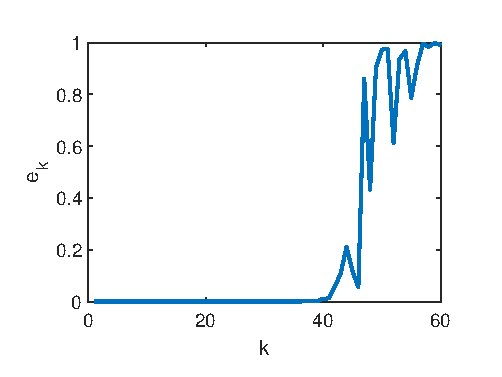
\includegraphics{qr-matlab-error.eps}
    \end{FigureCenter}


    图中显示了 $ q_{k} $ 与前面列之间的正交性的偏差:

    \begin{equation}
    e_{k}=\max _{1 \leq i<k}\left|q_{i}^{T} q_{k}\right|, \quad k=2, \ldots, n
    \end{equation}

    失去正交性是由于\textbf{浮点数存储的舍入误差}.

    修正的Gram-Schmidt则改为每次只减去一个投影,以减少舍入误差。

    \begin{lstlisting}[caption=modified Gram-Schmidt算法,language=matlab]
for j = 1:n
    v=A(:,j);
    for i=1:j-1
        R(i,j)=Q(:,i)'*v;
        v=v-R(i,j)*Q(:,i);
    end
    R(j,j)= norm(v);
    Q(:,j)=v/R(j,j);
end
    \end{lstlisting}

    \begin{algorithm}[htbp]
        \KwIn{矩阵$A$}
        \KwOut{QR分解得到的矩阵$Q$、$R$}
        \caption{Modified Gram-Schmidt Algorithm}
        \For(){$j=1$ to $n$}{
            $v={\tilde{q} }_j =a_j$\;
            \For(){$i=1$ to $j-1$}{
                $R_{ij} = q_i^T v$\;
                $v = v - R_{ij} q_i$\;
            }
            $R_{ jj} ={\left\|{\tilde{q} }_j \right\|}_2$\;
            $q_j =\left(\frac{1}{R_{jj} }\right){\tilde{q} }_j$\;

        }
    \end{algorithm}


    \begin{FigureCenter}{在同一组数据中使用修正Gram-Schmidt算法求得的误差,$e_{k}=\max _{1 \leq i<k}\left|q_{i}^{T} q_{k}\right|,  k=2, \ldots, n$}
        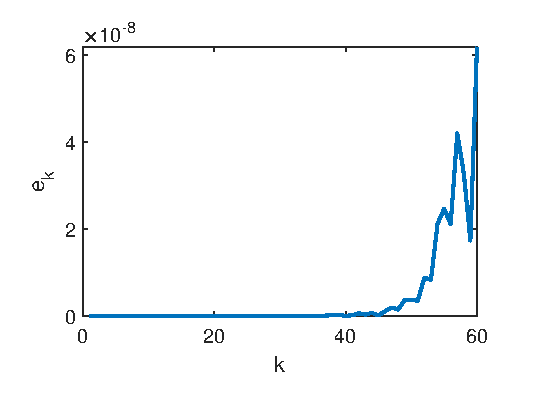
\includegraphics{modified-qr-matlab-error.eps}
    \end{FigureCenter}

    从图中可以看出,修正Gram-Schmidt算法的误差更小。
\end{example}

\section{QR Decomposition Using Householder Transformation}

Householder算法是QR分解常用的算法(\textsc{MATLAB}和\textsc{Julia}中的\verb|qr|函数)。与Gram-Schmidt相比,对舍入误差更有鲁棒性。

Householder算法计算一个“完整的”QR分解:
\begin{equation} A_{m \times n}=\left[\begin{array}{ll}Q_{m \times n} & \tilde{Q}_{m \times (m-n)}\end{array}\right]\left[\begin{array}{l}R_{n  \times  n} \\ 0_{(m-n) \times n}\end{array}\right], \quad\left[\begin{array}{ll}Q & \tilde{Q}\end{array}\right]  是列正交的矩阵\end{equation}

\begin{proof}
    \begin{equation}
    \begin{aligned}
        A&=\left[\begin{array}{ll}Q & \tilde{Q}\end{array}\right]\left[\begin{array}{l}R \\ 0\end{array}\right]\\
        &=QR + \tilde{Q} 0 \\ 
        & = QR
    \end{aligned}
    \end{equation}
\end{proof}

where $ R $ is an $ n \times n $ upper triangular matrix, $0$ is an $ (m-n) \times n $ zero matrix, $ Q  $ is $ m \times n,\tilde{Q} $ is $ m \times(m-n) $, and $ Q $ and $ \tilde{Q} $ both have orthogonal columns. 

\begin{remark}
    $A \in \mathfrak{R}^{m \times n}, m \ge n$,当$m < n$时列线性相关,无法进行QR分解。
\end{remark}



完整的$Q$因子被构造成正交矩阵的乘积:
\begin{equation}
\left[\begin{array}{ll}
Q & \tilde{Q}
\end{array}\right]=H_{1} H_{2} \cdots H_{n}
\end{equation}
每个 $ H_{i} \in \mathfrak{R}^{m \times m} $ 是对称正交的Householder矩阵。



\subsection{Householder Matrix}

\begin{theorem}
    $ H=I-2 v v^{T} $, 其中 $ \|v\|_{2}=1 $, $ H x $ 是 $ x $ 关于超平面 $ \left\{u \mid v^{T} u=0\right\} $ 反对称。
\end{theorem}

\begin{theorem}
    $ H $ 是对称的。
    \begin{equation} H^{T}=H \end{equation}
\end{theorem}
    
\begin{theorem}
    $ H $ \textbf{是标准正交的}.
\begin{equation} H^{T} H=I \end{equation}
\end{theorem}

\subsection{反射算子的几何图示}
\begin{FigureCenter}{Reflection of $x$}
    

\tikzset{every picture/.style={line width=0.75pt}} %set default line width to 0.75pt        

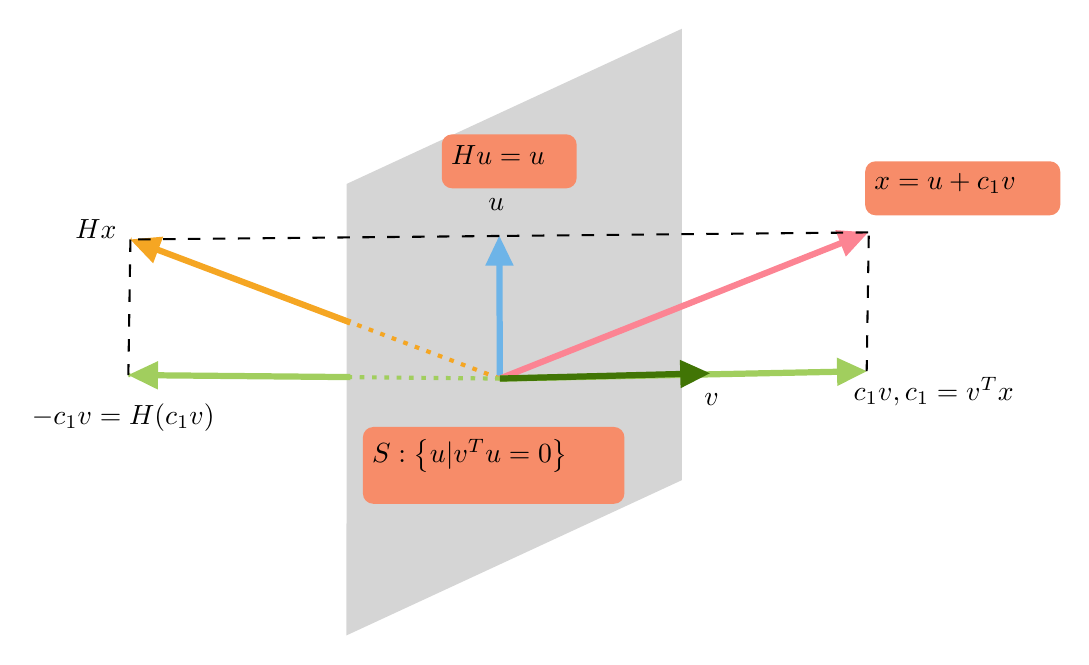
\begin{tikzpicture}[x=0.75pt,y=0.75pt,yscale=-1,xscale=1]
%uncomment if require: \path (0,334); %set diagram left start at 0, and has height of 334

%Shape: Parallelogram [id:dp7838939596356449] 
\draw  [color={rgb, 255:red, 0; green, 0; blue, 0 }  ,draw opacity=0 ][fill={rgb, 255:red, 213; green, 213; blue, 213 }  ,fill opacity=1 ] (401.66,234.62) -- (240.09,309.42) -- (240.16,91.9) -- (401.73,17.11) -- cycle ;
%Straight Lines [id:da6147749821862796] 
\draw [color={rgb, 255:red, 109; green, 180; blue, 232 }  ,draw opacity=1 ][line width=2.25]    (314,185.67) -- (313.74,121.96) ;
\draw [shift={(313.72,116.96)}, rotate = 449.76] [fill={rgb, 255:red, 109; green, 180; blue, 232 }  ,fill opacity=1 ][line width=0.08]  [draw opacity=0] (14.29,-6.86) -- (0,0) -- (14.29,6.86) -- cycle    ;
%Straight Lines [id:da41583656892756826] 
\draw [color={rgb, 255:red, 245; green, 166; blue, 35 }  ,draw opacity=1 ][line width=1.5]  [dash pattern={on 1.69pt off 2.76pt}]  (314,185.67) -- (136,118.67) ;
%Straight Lines [id:da16926502578383218] 
\draw [color={rgb, 255:red, 245; green, 166; blue, 35 }  ,draw opacity=1 ][line width=2.25]    (242,158.67) -- (140.68,120.43) ;
\draw [shift={(136,118.67)}, rotate = 380.66999999999996] [fill={rgb, 255:red, 245; green, 166; blue, 35 }  ,fill opacity=1 ][line width=0.08]  [draw opacity=0] (14.29,-6.86) -- (0,0) -- (14.29,6.86) -- cycle    ;
%Straight Lines [id:da9973542879627482] 
\draw [color={rgb, 255:red, 252; green, 132; blue, 147 }  ,draw opacity=1 ][line width=2.25]    (314,185.67) -- (486.78,117.1) ;
\draw [shift={(491.43,115.25)}, rotate = 518.35] [fill={rgb, 255:red, 252; green, 132; blue, 147 }  ,fill opacity=1 ][line width=0.08]  [draw opacity=0] (14.29,-6.86) -- (0,0) -- (14.29,6.86) -- cycle    ;
%Straight Lines [id:da33840798922577653] 
\draw [color={rgb, 255:red, 161; green, 206; blue, 94 }  ,draw opacity=1 ][line width=1.5]  [dash pattern={on 1.69pt off 2.76pt}]  (314,185.67) -- (135,183.96) ;
%Straight Lines [id:da7106398441661397] 
\draw [color={rgb, 255:red, 161; green, 206; blue, 94 }  ,draw opacity=1 ][line width=2.25]    (242,184.96) -- (140,184.01) ;
\draw [shift={(135,183.96)}, rotate = 360.53999999999996] [fill={rgb, 255:red, 161; green, 206; blue, 94 }  ,fill opacity=1 ][line width=0.08]  [draw opacity=0] (14.29,-6.86) -- (0,0) -- (14.29,6.86) -- cycle    ;
%Straight Lines [id:da3197102975021888] 
\draw [color={rgb, 255:red, 161; green, 206; blue, 94 }  ,draw opacity=1 ][line width=2.25]    (314,185.67) -- (485.73,182.21) ;
\draw [shift={(490.73,182.11)}, rotate = 538.85] [fill={rgb, 255:red, 161; green, 206; blue, 94 }  ,fill opacity=1 ][line width=0.08]  [draw opacity=0] (14.29,-6.86) -- (0,0) -- (14.29,6.86) -- cycle    ;
%Straight Lines [id:da07789590448724115] 
\draw  [dash pattern={on 4.5pt off 4.5pt}]  (136,118.67) -- (135,183.96) ;
%Straight Lines [id:da5486690595919534] 
\draw  [dash pattern={on 4.5pt off 4.5pt}]  (313.72,116.96) -- (136,118.67) ;
%Straight Lines [id:da1919773551202424] 
\draw  [dash pattern={on 4.5pt off 4.5pt}]  (491.43,115.25) -- (313.72,116.96) ;
%Straight Lines [id:da06488229558680647] 
\draw  [dash pattern={on 4.5pt off 4.5pt}]  (491.73,116.81) -- (490.99,164.67) -- (490.73,182.11) ;
%Straight Lines [id:da5187220488118582] 
\draw [color={rgb, 255:red, 65; green, 117; blue, 5 }  ,draw opacity=1 ][line width=2.25]    (314,185.67) -- (410.18,183.23) ;
\draw [shift={(415.18,183.11)}, rotate = 538.55] [fill={rgb, 255:red, 65; green, 117; blue, 5 }  ,fill opacity=1 ][line width=0.08]  [draw opacity=0] (14.29,-6.86) -- (0,0) -- (14.29,6.86) -- cycle    ;

% Text Node
\draw (108,107.4) node [anchor=north west][inner sep=0.75pt]    {$\boldsymbol{Hx}$};
% Text Node
\draw (307,97.4) node [anchor=north west][inner sep=0.75pt]    {$u$};
% Text Node
\draw  [color={rgb, 255:red, 12; green, 12; blue, 12 }  ,draw opacity=0 ][fill={rgb, 255:red, 247; green, 140; blue, 105 }  ,fill opacity=1 ]  (286,73) .. controls (286,70.24) and (288.24,68) .. (291,68) -- (346,68) .. controls (348.76,68) and (351,70.24) .. (351,73) -- (351,89) .. controls (351,91.76) and (348.76,94) .. (346,94) -- (291,94) .. controls (288.24,94) and (286,91.76) .. (286,89) -- cycle  ;
\draw (289,72) node [anchor=north west][inner sep=0.75pt]   [align=left] {$\displaystyle \boldsymbol{Hu=u}$};
% Text Node
\draw (87,196.4) node [anchor=north west][inner sep=0.75pt]    {$\boldsymbol{-c_{1} v=H( c_{1} v)}$};
% Text Node
\draw  [color={rgb, 255:red, 0; green, 0; blue, 0 }  ,draw opacity=0 ][fill={rgb, 255:red, 247; green, 140; blue, 105 }  ,fill opacity=1 ]  (490,86) .. controls (490,83.24) and (492.24,81) .. (495,81) -- (579,81) .. controls (581.76,81) and (584,83.24) .. (584,86) -- (584,102) .. controls (584,104.76) and (581.76,107) .. (579,107) -- (495,107) .. controls (492.24,107) and (490,104.76) .. (490,102) -- cycle  ;
\draw (493,85.4) node [anchor=north west][inner sep=0.75pt]    {$\boldsymbol{x=u+c_{1} v}$};
% Text Node
\draw  [color={rgb, 255:red, 0; green, 0; blue, 0 }  ,draw opacity=0 ][fill={rgb, 255:red, 247; green, 140; blue, 105 }  ,fill opacity=1 ]  (248,214) .. controls (248,211.24) and (250.24,209) .. (253,209) -- (369,209) .. controls (371.76,209) and (374,211.24) .. (374,214) -- (374,241) .. controls (374,243.76) and (371.76,246) .. (369,246) -- (253,246) .. controls (250.24,246) and (248,243.76) .. (248,241) -- cycle  ;
\draw (251,213.4) node [anchor=north west][inner sep=0.75pt]    {$S:\left\{\boldsymbol{u} |\boldsymbol{v}^{T}\boldsymbol{u} =0\right\}$};
% Text Node
\draw (483,183.4) node [anchor=north west][inner sep=0.75pt]    {$\boldsymbol{c_{1} v} ,\boldsymbol{c_{1} =v}^{T}\boldsymbol{x}$};
% Text Node
\draw (411,191.4) node [anchor=north west][inner sep=0.75pt]    {$\boldsymbol{v}$};


\end{tikzpicture}
\end{FigureCenter}

可以证明

\begin{theorem}
    $Hx$是$x$的关于超平面$ \left\{u \mid v^{T} u=0\right\} $镜面对称。
\end{theorem}



\begin{proof}
    \begin{equation}\begin{aligned}
        Hv &= (I-2 v v^{T}) (c_1 v) \\
        &= c_1 v - 2 v v^T c_1 v \\
        & = c_1 v - 2 c_1 v v^T v \\
        & = -c_1 v
    \end{aligned}\end{equation}

    \begin{equation}\begin{aligned}
        Hu &= (I - 2 v v^T) u \\
        &= u - 2 v v^T u \\
        & = u \quad (v^T u = 0) 
    \end{aligned}\end{equation}

    \begin{equation}\begin{aligned}
        Hx &= H(u + c_1v) \\
        &= u - c_1 v \\
        &= x - 2(v^Tx)v
    \end{aligned}\end{equation}
\end{proof}

\begin{corollary}
    矩阵向量积 $ H x $ 能化简为
\begin{equation}
H x=x-2\left(v^{T} x\right) v
\end{equation}
\end{corollary}


\subsubsection{$Hx$的算法复杂度}
    \label{complexity:Hx}

    如果 $ v $ 和 $ x $ 的长度是 $ p $, 复杂度是 $ 4 p $ flops.


\subsection{构造反射算子}

给定非零$p$维向量 $ y=\left(y_{1}, y_{2}, \ldots, y_{p}\right) $, 定义

\begin{definition}
    \begin{equation}w=\left[\begin{array}{c}
        y_{1}+\operatorname{sign}\left(y_{1}\right)\|y\|_{2} \\
        y_{2} \\
        \vdots \\
        y_{p}
        \end{array}\right]\end{equation}

    \begin{equation}v=\frac{1}{\|w\|_{2}} w\end{equation}

    $\operatorname{sign}(x)$ 是符号函数, $\operatorname{sign}(0)=0$.
\end{definition}

\begin{theorem}
    向量 $ w $ 满足 \begin{equation} \|w\|_{2}^{2}=2 y^{T} w \end{equation}
\end{theorem}

\begin{equation}
\begin{aligned}
    \|w\|_{2}^{2}&=w^{T} w\\
    &=2\left(\|y\|_{2}^{2}+\left|y_{1}\right|\|y\|_{2}\right)\\
    &=2 y^{T}\left(y+\operatorname{sign}\left(y_{1}\right)\|y\|_{2} e_{1}\right)\\
    &=2 y^{T} w 
\end{aligned}
\end{equation}

\begin{definition}[Constructed Householder Matrix]
将$y$变换为单位基向量$e=[1,0,0,\cdots,0]^T$乘以一个常数的Householder矩阵为

    \begin{equation} H=I-2 \frac{w w^{T}}{\|w\|_{2}^{2}} \end{equation}
\end{definition}

\begin{proof}
    \begin{equation} H=I-2 v v^{T}=I-2 \frac{w w^{T}}{\|w\|_{2}^{2}} \quad(v=\frac{1}{\|w\|_{2}} w) \end{equation}
\end{proof}

\begin{theorem}
    Householder矩阵 $ H=I-2 v v^{T}=I-2 \frac{w w^{T}}{\|w\|_{2}^{2}} $ 将 $ y $ 映射为

   \begin{equation} H y = \left[\begin{array}{c}-\operatorname{sign}\left(y_{1}\right)\|y\|_{2} \\ 0 \\ \vdots \\ 0\end{array}\right] = r_1 \end{equation}
\end{theorem}


\begin{proof}
    \begin{equation} 
\begin{aligned}
    H y&=y-\frac{2\left(w^{T} y\right)}{\|w\|_{2}^{2}} w\\
    &=y-w\\
    &=-\operatorname{sign}\left(y_{1}\right)\|y\|_{2} e_{1}\\
    &=\left[\begin{array}{c}-\operatorname{sign}\left(y_{1}\right)\|y\|_{2} \\ 0 \\ \vdots \\ 0\end{array}\right]
\end{aligned}
 \end{equation}
\end{proof}

即Householder变换的结果$Hy$只保留第一个元素的值,其余元素的值变为0. 又因为$H$是正交、对称的,它与QR分解求解$R$有一定联系。

\subsubsection{构造的Householder矩阵几何意义}


\begin{FigureCenter}{构造的Householder矩阵的几何意义}
   

\tikzset{every picture/.style={line width=0.75pt}} %set default line width to 0.75pt        

\begin{tikzpicture}[x=0.75pt,y=0.75pt,yscale=-1,xscale=1]
%uncomment if require: \path (0,341); %set diagram left start at 0, and has height of 341

%Straight Lines [id:da029865045800250956] 
\draw    (118.48,198.47) -- (513.53,197.71) ;
%Straight Lines [id:da7648219943630132] 
\draw    (249.95,81.42) -- (422.95,297.42) ;
%Straight Lines [id:da0029727641306782626] 
\draw [color={rgb, 255:red, 252; green, 132; blue, 147 }  ,draw opacity=1 ][line width=2.25]    (344.25,197.82) -- (370.82,84.25) ;
\draw [shift={(371.96,79.38)}, rotate = 463.17] [fill={rgb, 255:red, 252; green, 132; blue, 147 }  ,fill opacity=1 ][line width=0.08]  [draw opacity=0] (14.29,-6.86) -- (0,0) -- (14.29,6.86) -- cycle    ;
%Straight Lines [id:da8143455838821552] 
\draw [color={rgb, 255:red, 245; green, 166; blue, 35 }  ,draw opacity=1 ][line width=2.25]    (344.25,197.82) -- (228.57,198.09) ;
\draw [shift={(223.57,198.11)}, rotate = 359.87] [fill={rgb, 255:red, 245; green, 166; blue, 35 }  ,fill opacity=1 ][line width=0.08]  [draw opacity=0] (14.29,-6.86) -- (0,0) -- (14.29,6.86) -- cycle    ;
%Straight Lines [id:da703987286749107] 
\draw  [dash pattern={on 4.5pt off 4.5pt}]  (297.77,138.74) -- (223.57,198.11) ;
%Straight Lines [id:da00886805291354964] 
\draw  [dash pattern={on 4.5pt off 4.5pt}]  (371.96,79.38) -- (297.77,138.74) ;
%Straight Lines [id:da1380735800367292] 
\draw [color={rgb, 255:red, 152; green, 195; blue, 245 }  ,draw opacity=1 ][line width=2.25]    (223.57,198.11) -- (368.05,82.5) ;
\draw [shift={(371.96,79.38)}, rotate = 501.34] [fill={rgb, 255:red, 152; green, 195; blue, 245 }  ,fill opacity=1 ][line width=0.08]  [draw opacity=0] (14.29,-6.86) -- (0,0) -- (14.29,6.86) -- cycle    ;
%Shape: Right Triangle [id:dp29057470922525686] 
\draw   (161,382.99) -- (208.53,431.62) -- (161,431.62) -- cycle ;

% Text Node
\draw (302.81,99.57) node [anchor=north west][inner sep=0.75pt]    {$w$};
% Text Node
\draw (175,208.4) node [anchor=north west][inner sep=0.75pt]    {$-\operatorname{sign}( y_{1}) \| y\| e_{1}$};
% Text Node
\draw (360.24,141.91) node [anchor=north west][inner sep=0.75pt]  [rotate=-357.61]  {$y$};
% Text Node
\draw (447,176) node [anchor=north west][inner sep=0.75pt]   [align=left] {坐标轴 $\displaystyle e_{1}$};
% Text Node
\draw (394,237) node [anchor=north west][inner sep=0.75pt]   [align=left] {超平面$\displaystyle \left\{x|w^{T} x=0\right\}$};


\end{tikzpicture}
\end{FigureCenter}


关于超平面 $ \left\{x \mid w^{T} x=0\right\} $, 其法向量$w,v$:
\begin{equation}
w=y+\operatorname{sign}\left(y_{1}\right)\|y\|_{2} e_{1},v=\frac{w}{\|w\|_{2}}
\end{equation}
反射算子$H$将 $ y $ 映射到向量 $ -\operatorname{sign}\left(y_{1}\right)\|y\|_{2} e_{1} $ .

\subsection{Householder三角化}

计算反射算子 $ H_{1}, \ldots, H_{n} $ 将$A$简化为上三角矩阵形式:
\begin{equation}
H_{n} H_{n-1} \cdots H_{1} A=\left[\begin{array}{l}
R \\
0
\end{array}\right]
\end{equation}


第$k$个步骤之后,矩阵 $ H_{k} H_{k-1} \ldots H_{1} A $ 具有以下结构:

\tikzset{every picture/.style={line width=0.75pt}} %set default line width to 0.75pt        
对于 $ i>j $ 和 $ j \leq k $, 第 $  {i},  {j} $ 个位置的元素为零。


\begin{FigureCenter}{The Structure of $ H_{k} H_{k-1} \ldots H_{1} A $}
    

\tikzset{every picture/.style={line width=0.75pt}} %set default line width to 0.75pt        

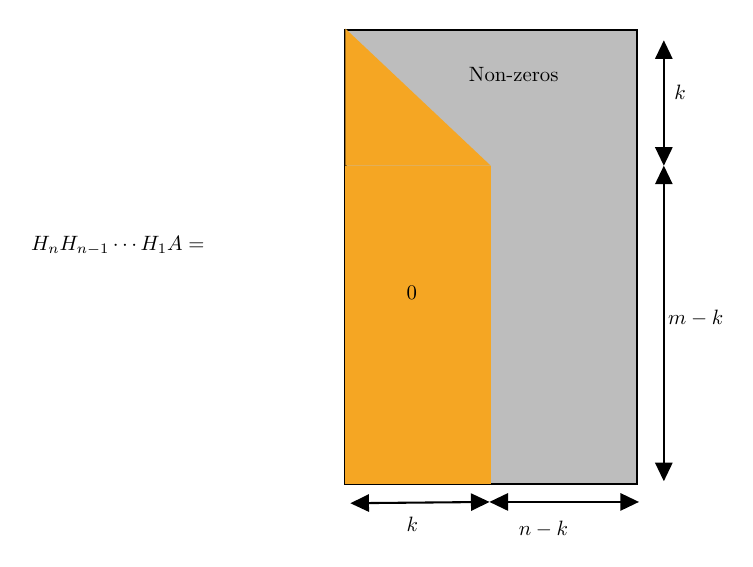
\begin{tikzpicture}[x=0.75pt,y=0.75pt,yscale=-1,xscale=1]
%uncomment if require: \path (0,300); %set diagram left start at 0, and has height of 300

%Shape: Rectangle [id:dp6272763265145869] 
\draw  [fill={rgb, 255:red, 189; green, 189; blue, 189 }  ,fill opacity=1 ] (313,30) -- (453.39,30) -- (453.39,248.71) -- (313,248.71) -- cycle ;
%Shape: Rectangle [id:dp1811444148627901] 
\draw  [color={rgb, 255:red, 0; green, 0; blue, 0 }  ,draw opacity=0 ][fill={rgb, 255:red, 245; green, 166; blue, 35 }  ,fill opacity=1 ] (313,95.38) -- (383,95.38) -- (383,248.71) -- (313,248.71) -- cycle ;
%Shape: Right Triangle [id:dp6024983200469929] 
\draw  [color={rgb, 255:red, 0; green, 0; blue, 0 }  ,draw opacity=0 ][fill={rgb, 255:red, 245; green, 166; blue, 35 }  ,fill opacity=1 ] (313,29.38) -- (383,95.38) -- (313,95.38) -- cycle ;

%Straight Lines [id:da17687674689557986] 
\draw    (466.39,38) -- (466.39,92.38) ;
\draw [shift={(466.39,95.38)}, rotate = 270] [fill={rgb, 255:red, 0; green, 0; blue, 0 }  ][line width=0.08]  [draw opacity=0] (8.93,-4.29) -- (0,0) -- (8.93,4.29) -- cycle    ;
\draw [shift={(466.39,35)}, rotate = 90] [fill={rgb, 255:red, 0; green, 0; blue, 0 }  ][line width=0.08]  [draw opacity=0] (8.93,-4.29) -- (0,0) -- (8.93,4.29) -- cycle    ;
%Straight Lines [id:da19218796013321793] 
\draw    (466.39,98.38) -- (466.39,244.38) ;
\draw [shift={(466.39,247.38)}, rotate = 270] [fill={rgb, 255:red, 0; green, 0; blue, 0 }  ][line width=0.08]  [draw opacity=0] (8.93,-4.29) -- (0,0) -- (8.93,4.29) -- cycle    ;
\draw [shift={(466.39,95.38)}, rotate = 90] [fill={rgb, 255:red, 0; green, 0; blue, 0 }  ][line width=0.08]  [draw opacity=0] (8.93,-4.29) -- (0,0) -- (8.93,4.29) -- cycle    ;
%Straight Lines [id:da4247865332087235] 
\draw    (318.39,257.97) -- (379.39,257.41) ;
\draw [shift={(382.39,257.38)}, rotate = 179.47] [fill={rgb, 255:red, 0; green, 0; blue, 0 }  ][line width=0.08]  [draw opacity=0] (8.93,-4.29) -- (0,0) -- (8.93,4.29) -- cycle    ;
\draw [shift={(315.39,258)}, rotate = 359.47] [fill={rgb, 255:red, 0; green, 0; blue, 0 }  ][line width=0.08]  [draw opacity=0] (8.93,-4.29) -- (0,0) -- (8.93,4.29) -- cycle    ;
%Straight Lines [id:da09293842736310576] 
\draw    (385.39,257.38) -- (451.39,257.38) ;
\draw [shift={(454.39,257.38)}, rotate = 180] [fill={rgb, 255:red, 0; green, 0; blue, 0 }  ][line width=0.08]  [draw opacity=0] (8.93,-4.29) -- (0,0) -- (8.93,4.29) -- cycle    ;
\draw [shift={(382.39,257.38)}, rotate = 0] [fill={rgb, 255:red, 0; green, 0; blue, 0 }  ][line width=0.08]  [draw opacity=0] (8.93,-4.29) -- (0,0) -- (8.93,4.29) -- cycle    ;

% Text Node
\draw (470.39,55.4) node [anchor=north west][inner sep=0.75pt]  [xscale=0.75,yscale=0.75]  {$k$};
% Text Node
\draw (467.39,163.78) node [anchor=north west][inner sep=0.75pt]  [xscale=0.75,yscale=0.75]  {$m-k$};
% Text Node
\draw (341.39,263.4) node [anchor=north west][inner sep=0.75pt]  [xscale=0.75,yscale=0.75]  {$k$};
% Text Node
\draw (395.39,265.4) node [anchor=north west][inner sep=0.75pt]  [xscale=0.75,yscale=0.75]  {$n-k$};
% Text Node
\draw (160.39,128.4) node [anchor=north west][inner sep=0.75pt]  [xscale=0.75,yscale=0.75]  {$H_{n} H_{n-1} \cdots H_{1} A=$};
% Text Node
\draw (341.39,152.4) node [anchor=north west][inner sep=0.75pt]  [xscale=0.75,yscale=0.75]  {$\boldsymbol{0}$};
% Text Node
\draw (371.39,47) node [anchor=north west][inner sep=0.75pt]  [xscale=0.75,yscale=0.75] [align=left] {Non-zeros};


\end{tikzpicture}     
\end{FigureCenter}

其过程如下:


\begin{equation} A=\left[\begin{array}{llllllll}X & X & X & X & X & X & X & X \\ X & X & X & X & X & X & X & X \\ X & X & X & X & X & X & X & X \\ X & X & X & X & X & X & X & X \\ X & X & X & X & X & X & X & X \\ X & X & X & X & X & X & X & X \\ X & X & X & X & X & X & X & X \\ X & X & X & X & X & X & X & X\end{array}\right] \end{equation}

在第一次处理之后,$A_1$第一列只剩下第一个元素不为0.

\begin{equation}H_1A = A_{1}=\left[\begin{array}{llllllll}X & X & X & X & X & X & X & X \\ 0 & X & X & X & X & X & X & X \\ 0 & X & X & X & X & X & X & X \\ 0 & X & X & X & X & X & X & X \\ 0 & X & X & X & X & X & X & X \\ 0 & X & X & X & X & X & X & X \\ 0 & X & X & X & X & X & X & X \\ 0 & X & X & X & X & X & X & X\end{array}\right] \end{equation}

第二次处理对于$H_1A_{2:m, 1:n}$($A_{1_{1:m, 1:n} }  $)进行处理。

\begin{equation}H_2A_1= A_{2}=\left[\begin{array}{cccccccc}X & X & X & X & X & X & X & X \\ 0 & X & X & X & X & X & X & X \\ 0 & 0 & X & X & X & X & X & X \\ 0 & 0 & X & X & X & X & X & X \\ 0 & 0 & X & X & X & X & X & X \\ 0 & 0 & X & X & X & X & X & X \\ 0 & 0 & X & X & X & X & X & X \\ 0 & 0 & X & X & X & X & X & X\end{array}\right] \end{equation}

以此类推,直至矩阵$A$变成上三角矩阵。


\begin{FigureCenter}{迭代计算过程中$A$的结构}
    \tikzset{every picture/.style={line width=0.75pt}} %set default line width to 0.75pt

    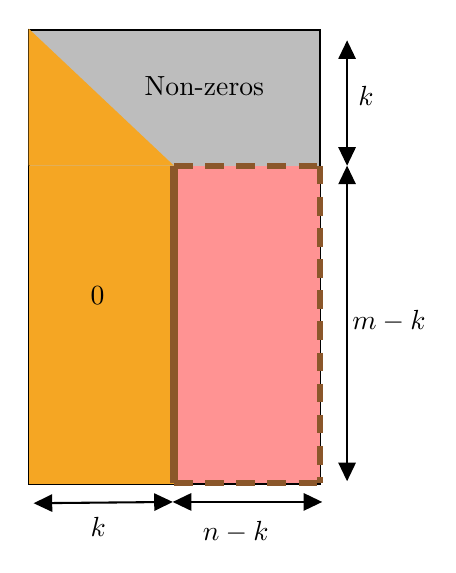
\begin{tikzpicture}[x=0.75pt,y=0.75pt,yscale=-1,xscale=1]
        %uncomment if require: \path (0,300); %set diagram left start at 0, and has height of 300
        
        %Shape: Rectangle [id:dp6871792923402225] 
        \draw  [fill={rgb, 255:red, 189; green, 189; blue, 189 }  ,fill opacity=1 ] (333,28) -- (473.39,28) -- (473.39,246.71) -- (333,246.71) -- cycle ;
        %Shape: Rectangle [id:dp8707939685410495] 
        \draw  [color={rgb, 255:red, 0; green, 0; blue, 0 }  ,draw opacity=0 ][fill={rgb, 255:red, 245; green, 166; blue, 35 }  ,fill opacity=1 ] (333,93.38) -- (403,93.38) -- (403,246.71) -- (333,246.71) -- cycle ;
        %Shape: Right Triangle [id:dp15297612966191965] 
        \draw  [color={rgb, 255:red, 0; green, 0; blue, 0 }  ,draw opacity=0 ][fill={rgb, 255:red, 245; green, 166; blue, 35 }  ,fill opacity=1 ] (333,27.38) -- (403,93.38) -- (333,93.38) -- cycle ;
        
        %Straight Lines [id:da37642223834770605] 
        \draw    (486.39,36) -- (486.39,90.38) ;
        \draw [shift={(486.39,93.38)}, rotate = 270] [fill={rgb, 255:red, 0; green, 0; blue, 0 }  ][line width=0.08]  [draw opacity=0] (8.93,-4.29) -- (0,0) -- (8.93,4.29) -- cycle    ;
        \draw [shift={(486.39,33)}, rotate = 90] [fill={rgb, 255:red, 0; green, 0; blue, 0 }  ][line width=0.08]  [draw opacity=0] (8.93,-4.29) -- (0,0) -- (8.93,4.29) -- cycle    ;
        %Straight Lines [id:da1511742331917798] 
        \draw    (486.39,96.38) -- (486.39,242.38) ;
        \draw [shift={(486.39,245.38)}, rotate = 270] [fill={rgb, 255:red, 0; green, 0; blue, 0 }  ][line width=0.08]  [draw opacity=0] (8.93,-4.29) -- (0,0) -- (8.93,4.29) -- cycle    ;
        \draw [shift={(486.39,93.38)}, rotate = 90] [fill={rgb, 255:red, 0; green, 0; blue, 0 }  ][line width=0.08]  [draw opacity=0] (8.93,-4.29) -- (0,0) -- (8.93,4.29) -- cycle    ;
        %Straight Lines [id:da9300057482807336] 
        \draw    (338.39,255.97) -- (399.39,255.41) ;
        \draw [shift={(402.39,255.38)}, rotate = 539.47] [fill={rgb, 255:red, 0; green, 0; blue, 0 }  ][line width=0.08]  [draw opacity=0] (8.93,-4.29) -- (0,0) -- (8.93,4.29) -- cycle    ;
        \draw [shift={(335.39,256)}, rotate = 359.47] [fill={rgb, 255:red, 0; green, 0; blue, 0 }  ][line width=0.08]  [draw opacity=0] (8.93,-4.29) -- (0,0) -- (8.93,4.29) -- cycle    ;
        %Straight Lines [id:da8104730881110522] 
        \draw    (405.39,255.38) -- (471.39,255.38) ;
        \draw [shift={(474.39,255.38)}, rotate = 180] [fill={rgb, 255:red, 0; green, 0; blue, 0 }  ][line width=0.08]  [draw opacity=0] (8.93,-4.29) -- (0,0) -- (8.93,4.29) -- cycle    ;
        \draw [shift={(402.39,255.38)}, rotate = 0] [fill={rgb, 255:red, 0; green, 0; blue, 0 }  ][line width=0.08]  [draw opacity=0] (8.93,-4.29) -- (0,0) -- (8.93,4.29) -- cycle    ;
        %Shape: Rectangle [id:dp3957948372583875] 
        \draw  [color={rgb, 255:red, 0; green, 0; blue, 0 }  ,draw opacity=0 ][fill={rgb, 255:red, 255; green, 147; blue, 147 }  ,fill opacity=1 ] (403,93.38) -- (473.39,93.38) -- (473.39,246.42) -- (403,246.42) -- cycle ;
        %Straight Lines [id:da6423678439002216] 
        \draw [color={rgb, 255:red, 139; green, 87; blue, 42 }  ,draw opacity=1 ][line width=3]    (403,93.38) -- (403,246.42) ;
        %Straight Lines [id:da15094884239960105] 
        \draw [color={rgb, 255:red, 139; green, 87; blue, 42 }  ,draw opacity=1 ][line width=2.25]  [dash pattern={on 6.75pt off 4.5pt}]  (403,93.38) -- (473.39,93.38) ;
        %Straight Lines [id:da6820341280353248] 
        \draw [color={rgb, 255:red, 139; green, 87; blue, 42 }  ,draw opacity=1 ][line width=2.25]  [dash pattern={on 6.75pt off 4.5pt}]  (473.39,93.38) -- (473.39,246.42) ;
        %Straight Lines [id:da3968465055227026] 
        \draw [color={rgb, 255:red, 139; green, 87; blue, 42 }  ,draw opacity=1 ][line width=2.25]  [dash pattern={on 6.75pt off 4.5pt}]  (403,246.42) -- (473.39,246.42) ;
        
        % Text Node
        \draw (490.39,53.4) node [anchor=north west][inner sep=0.75pt]    {$k$};
        % Text Node
        \draw (487.39,161.78) node [anchor=north west][inner sep=0.75pt]    {$m-k$};
        % Text Node
        \draw (361.39,261.4) node [anchor=north west][inner sep=0.75pt]    {$k$};
        % Text Node
        \draw (415.39,263.4) node [anchor=north west][inner sep=0.75pt]    {$n-k$};
        % Text Node
        \draw (361.39,150.4) node [anchor=north west][inner sep=0.75pt]    {$\boldsymbol{0}$};
        % Text Node
        \draw (387.39,49) node [anchor=north west][inner sep=0.75pt]   [align=left] {Non-zeros};
        
        
        \end{tikzpicture}
\end{FigureCenter}

\subsection{Householder-QR Algorithm}

\begin{algorithm}[htbp]
    \caption{QR Decomposition Using Householder Transformation}
    \KwIn{Matrix $A$}
    \KwOut{$v_1, \cdots, v_n, v_k \in \mathfrak{R}^{m-k+1} $ ($Q$), $A=
    \left[\begin{array}{c}
    R \\
    0
    \end{array}\right]$ ($R$)
    }

    \For(){$k$ in $1:n$}{
        令 $ y=A_{k: m, k} \in \mathfrak{R}^{m-k+1} $, 计算向量 $ v_{k} $
    \begin{equation} w=y+\operatorname{sign}\left(y_{1}\right)\|y\| e_{1}\end{equation}
    \begin{equation} v_{k}=\frac{1}{\|w\|} w \end{equation}\;

    将 $ A_{k: m, k: n} \in \mathfrak{R}^{(m-k+1) \times(n-k+1)} $ 与反射矩阵 $ I-2 v_{k} v_{k}^{T} $ 相乘
    \begin{equation} A_{k: m, k: n}:=A_{k: m, k: n}-2 v_{k}\left(v_{k}^{T} A_{k: m, k: n}\right) \end{equation}\;
    }
\end{algorithm}

\begin{theorem}
     在算法步骤2中,将 $ A_{k: m, k: n} $ 与反射算子 $ I-2 v_{k} v_{k}^{T} $ 相乘

    \begin{equation} \left(I-2 v_{k} v_{k}^{T}\right) A_{k: m, k: n}=A_{k: m, k: n}-2 v_{k}\left(v_{k}^{T} A_{k: m, k: n}\right) \end{equation}

    等价于用 $ H_{k} \in \mathfrak{R}^{m \times m} $ 乘以 $ A \in \mathfrak{R}^{m \times n}  $

    \begin{equation} H_{k}=\left[\begin{array}{cc}I & 0 \\ 0 & I-2 v_{k} v_{k}^{T}\end{array}\right]=I-2\left[\begin{array}{c}0 \\ v_{k}\end{array}\right]\left[\begin{array}{l}0 \\ v_{k}\end{array}\right]^{T} \end{equation}
\end{theorem}

   

算法的最终结果将下列矩阵来代替 $ A\in \mathfrak{R}^{m \times n}  $
\begin{equation}
\left[\begin{array}{c}
R \\
0
\end{array}\right]
\end{equation}

返回向量 $ v_{1}, \ldots, v_{n} $, 其中 $ v_{k} $ 的长度为 $ m-k+1 $ .

\subsection{Complexity of Householder Algorithm}
\label{complexity:householder}

\begin{equation} H_{k}=\left[\begin{array}{cc}I & 0 \\ 0 & I-2 v_{k} v_{k}^{T}\end{array}\right]=I-2\left[\begin{array}{c}0 \\ v_{k}\end{array}\right]\left[\begin{array}{l}0 \\ v_{k}\end{array}\right]^{T} \end{equation}

第$k$次循环时,$v_k \in \mathfrak{R}^{m - k + 1}$.

Householder方法第$k$次循环的复杂度:

\begin{itemize}
    \item 构造$v$需要$4p = 4(m - k + 1)$ flops.
    \item $ v_{k}^{T} A_{k: m, k: n} $ 的乘积: $ (2({m}-{k}+1)-1)({n}-{k}+1) $ flops
    \item $ v_{k} $ 的外积: $ (m-k+1)(n-k+1) $ flops
    \item $ A_{k: m, k: n} $ 的减法: $ ({m}-{k}+1)({n}-{k}+1) $ flops
\end{itemize}

除去构造$v$所需要的flops总和是$ 4({m}-{k}+1)({n}-{k}+1) $ flops,加上构造$v$需要的flops,所以第$k$次循环的总和: $ 4({m}-{k}+1)({n}-{k}+2) $ flops

\begin{theorem}
    计算 $ R $ 和 $ v_{1}, \ldots, v_{n} $ 的总复杂度

\begin{equation} \begin{aligned} \sum_{k=1}^{n} 4(m-k+1)(n-k+\boldsymbol{2}) & \approx \int_{0}^{n} 4(m-t)(n-t+1) d t \\ & \approx 2 m n^{2}-\frac{2}{3} n^{3} \text { flops } \end{aligned} \end{equation}
\end{theorem}



\subsection{An Example for Householder Algorithm}

\begin{problem}
    \begin{equation} A=\left[\begin{array}{rrr}-1 & -1 & 1 \\ 1 & 3 & 3 \\ -1 & -1 & 5 \\ 1 & 3 & 7\end{array}\right]=H_{1} H_{2} H_{3}\left[\begin{array}{l}R \\ 0\end{array}\right] \end{equation}

    计算反射算子 $ H_{1}, H_{2}, H_{3} $ 来将矩阵$A$三角化

    \begin{equation} H_{3} H_{2} H_{1} A=\left[\begin{array}{ccc}R_{11} & R_{12} & R_{13} \\ 0 & R_{22} & R_{23} \\ 0 & 0 & R_{33} \\ 0 & 0 & 0\end{array}\right] \end{equation}

    $R$的第一列:计算将$A$的第一列映射到$e_1$乘积的反射算子

    \begin{equation}
y=\left[\begin{array}{r}
-1 \\
1 \\
-1 \\
1
\end{array}\right], \quad w=y-\|y\|_{2} e_{1}=\left[\begin{array}{r}
-3 \\
1 \\
-1 \\
1
\end{array}\right], \quad v_{1}=\frac{1}{\|w\|_{2}} w=\frac{1}{2 \sqrt{3}}\left[\begin{array}{r}
-3 \\
1 \\
-1 \\
1
\end{array}\right]
\end{equation}

用 $I-2 v_{1} v_{1}^{T}$ 和$A$的乘积代替$A$:
\begin{equation}
A:=\left(I-2 v_{1} v_{1}^{T}\right) A=\left[\begin{array}{ccc}
2 & 4 & 2 \\
0 & 4 / 3 & 8 / 3 \\
0 & 2 / 3 & 16 / 3 \\
0 & 4 / 3 & 20 / 3
\end{array}\right]
\end{equation}

$R$的第二列:计算将 $ A_{2: 4,2} $ 映射到 $ e_{1} $ 乘积的反射算子

\begin{equation}y=\left[\begin{array}{l}
    4 / 3 \\
    2 / 3 \\
    4 / 3
    \end{array}\right], \quad w=y+\|y\|_{2} e_{1}=\left[\begin{array}{r}
    10 / 3 \\
    2 / 3 \\
    4 / 3
    \end{array}\right], \quad v_{2}=\frac{1}{\|w\|_{2}} w=\frac{1}{\sqrt{30}}\left[\begin{array}{l}
    5 \\
    1 \\
    2
    \end{array}\right]
\end{equation}

用 $I-2 v_{2} v_{2}^{T}$ 和 $A_{2: 4,2: 3}$ 的乘积代替 $A_{2: 4,2: 3}$ :
\begin{equation}
A:=\left[\begin{array}{cc}
1 & 0 \\
0 & I-2 v_{2} v_{2}^{T}
\end{array}\right] A=\left[\begin{array}{rrr}
2 & 4 & 2 \\
0 & -2 & -8 \\
0 & 0 & 16 / 5 \\
0 & 0 & 12 / 5
\end{array}\right]
\end{equation}

$R$的第三列:计算将$ A_{3: 4,3} $映射到$e_1$乘积的反射算子

\begin{equation}y=\left[\begin{array}{l}
    16 / 5 \\
    12 / 5
    \end{array}\right], \quad w=y+\|y\|_{2} e_{1}=\left[\begin{array}{c}
    36 / 5 \\
    12 / 5
    \end{array}\right], \quad v_{3}=\frac{1}{\|w\|_{2}} w=\frac{1}{\sqrt{10}}\left[\begin{array}{l}
    3 \\
    1
    \end{array}\right]
\end{equation}

用 $I-2 v_{3} v_{3}^{T}$ 和 $A_{3: 4,3}$ 的乘积代替 $A_{3: 4,3}$ :
\begin{equation}
A:=\left[\begin{array}{cc}
I & 0 \\
0 & I-2 v_{3} v_{3}^{T}
\end{array}\right] A=\left[\begin{array}{rrr}
2 & 4 & 2 \\
0 & -2 & -8 \\
0 & 0 & -4 \\
0 & 0 & 0
\end{array}\right]
\end{equation}

总的求解式为

    \begin{equation} \begin{aligned} H_{3} H_{2} H_{1} A &=\left[\begin{array}{cc}I_{2} & 0 \\ 0 & I_{2}-2 v_{3} v_{3}^{T}\end{array}\right]\left[\begin{array}{cc}I_{1} & 0 \\ 0 & I_{3}-2 v_{2} v_{2}^{T}\end{array}\right]\left(I_{4}-2 v_{1} v_{1}^{T}\right) A \\ &=\left[\begin{array}{cc}I_{2} & 0 \\ 0 & I_{2}-2 v_{3} v_{3}^{T}\end{array}\right]\left[\begin{array}{cc}I_{1} & 0 \\ 0 & I_{3}-2 v_{2} v_{2}^{T}\end{array}\right]\left[\begin{array}{ccc}2 & 4 & 2 \\ 0 & 4 / 3 & 8 / 3 \\ 0 & 2 / 3 & 16 / 3 \\ 0 & 4 / 3 & 20 / 3\end{array}\right] \\ &=\left[\begin{array}{cc}I_{2} & 0 \\ 0 & I_{2}-2 v_{3} v_{3}^{T}\end{array}\right]\left[\begin{array}{rrr}2 & 4 & 2 \\ 0 & -2 & -8 \\ 0 & 0 & 16 / 5 \\ 0 & 0 & 12 / 5\end{array}\right] \\ &=\left[\begin{array}{rrr}2 & 4 & 2 \\ 0 & -2 & -8 \\ 0 & 0 & -4 \\ 0 & 0 & 0\end{array}\right] \end{aligned} \end{equation}
\end{problem}



\section{Householder变换进行QR分解的 $Q$ 因子}

Householder算法返回向量 $ v_{1}, \ldots, v_{n} $, 其定义为:

\begin{definition}[ $ v_{1}, \ldots, v_{n} $ 的完整表示]
   \begin{equation}
\left[\begin{array}{ll}
Q & \tilde{Q}
\end{array}\right]=H_{1} H_{2} \cdots H_{n}
\end{equation} 
\end{definition}

通常不需计算矩阵 $ \left[\begin{array}{ll}Q & \tilde{Q}\end{array}\right] $ .向量 $ v_{1}, \ldots, v_{n} $ 是 $ \left[\begin{array}{ll}Q & \tilde{Q}\end{array}\right] $ 简单表示(economical representation).

\begin{theorem}
    $ \left[\begin{array}{ll}Q & \tilde{Q}\end{array}\right] $ 或其转置的乘积可以计算为:
\begin{equation}
\begin{array}{c}
{\left[\begin{array}{cc}
Q & \tilde{Q}
\end{array}\right] x=H_{1} H_{2} \cdots H_{n} x} \\
{\left[\begin{array}{ll}
Q & \tilde{Q}
\end{array}\right]^{T} y=H_{n} H_{n-1} \cdots H_{1} y}
\end{array}
\end{equation}
\end{theorem}

\subsection{Multiplication with $Q$ factor}

\begin{definition}[矩阵-向量积 $ H_{k} x $]
    矩阵-向量积 $ H_{k} x $ 定义为:
\begin{equation}
H_{k} x=\left[\begin{array}{cc}
I_{k-1} & 0 \\
0 & I-2 v_{k} v_{k}^{T}
\end{array}\right]\left[\begin{array}{c}
x_{1: k-1} \\
x_{k: m}
\end{array}\right]=\left[\begin{array}{c}
x_{1: k-1} \\
x_{k: m}-2\left(v_{k}^{T} x_{k: m}\right) v_{k}
\end{array}\right]
\end{equation}
\end{definition}

\subsection{矩阵-向量积 $ H_{k} x $算法复杂度}
\label{complexity:Hkx}

$ H_{k} x $ 乘积的复杂度为: $ 4( {m}- {k}+1) $ flops.

$H_{1} H_{2}, \ldots H_{n} $或其转置的乘积的复杂度为: 

\begin{equation} \sum_{k=1}^{n} 4(m-k+1) \approx 4 m n-2 n^{2}  \text{ flops}\end{equation}

其复杂度约等于$m \times n$矩阵的矩阵-向量乘积($2mn$ flops). 


\section{Fast Orthogonalization (Givens and Householder)}

\begin{remark}
    This section is quoted from \cite{Strang1993IntroductionTL}.
\end{remark}

There are three ways to reach the important factorization $A=Q R$. 

\textbf{Gram-Schmidt} works to find the orthonormal vectors in $Q .$ Then $R$ is upper triangular because of the order of Gram-Schmidt steps. 

Now we look at better methods (Householder and Givens), which use a product of specially simple $Q$'s that we know are orthogonal.

Elimination gives $A=L U$, orthogonalization gives $A=Q R$. We don't want a triangular $L$, we want an orthogonal $Q$. $L$ is a product of $E$'s from elimination, with 1's on the diagonal and the multiplier $\ell_{i j}$ below. \textbf{$Q$ will be a product of orthogonal matrices.}

There are two simple orthogonal matrices to take the place of the $E$'s. The \term{reflection matrices} $I-2 \boldsymbol{u} \boldsymbol{u}^{ {T}}$ are named after \textit{Householder}. The \term{plane rotation matrices} are named after \textit{Givens}. The simple matrix that rotates the $x y$ plane by $\theta$ is $Q_{21}$:  

\begin{definition}[Givens Rotation in the 1-2 plane]
    \begin{equation}Q_{21}=\left[\begin{array}{crc}
        \cos \theta & -\sin \theta & 0 \\
        \sin \theta & \cos \theta & 0 \\
        0 & 0 & 1
        \end{array}\right]\end{equation}
\end{definition}

Use $Q_{21}$ the way you used $E_{21}$, to produce a zero in the $(2,1)$ position. That determines the angle $\theta$. Bill Hager gives this example in Applied Numerical Linear Algebra:

\begin{example}[使用Givens进行QR分解]
    \begin{equation}
    Q_{21} A=\left[\begin{array}{rrr}
    .6 & .8 & 0 \\
    -.8 & .6 & 0 \\
    0 & 0 & 1
    \end{array}\right]\left[\begin{array}{rrr}
    90 & -153 & 114 \\
    120 & -79 & -223 \\
    200 & -40 & 395
    \end{array}\right]=\left[\begin{array}{crr}
    150 & -155 & -110 \\
    \mathbf{0} & 75 & -225 \\
    200 & -40 & 395
    \end{array}\right]
    \end{equation}

    The zero came from $-8(90)+.6(120)$. No need to find $\theta$, what we needed was $\cos \theta$
\begin{equation}
\cos \theta=\frac{90}{\sqrt{90^{2}+120^{2}}} \quad \text { and } \quad \sin \theta=\frac{-120}{\sqrt{90^{2}+120^{2}}}
\end{equation}

Now we attack the $(3,1)$ entry. The rotation will be in rows and columns 3 and 1 . The numbers $\cos \theta$ and $\sin \theta$ are determined from 150 and 200 , instead of 90 and 120 .
\begin{equation}
Q_{31} Q_{21} A=\left[\begin{array}{rrr}
.6 & 0 & .8 \\
0 & 1 & 0 \\
-.8 & 0 & .6
\end{array}\right]\left[\begin{array}{rrr}
150 & \cdot & \cdot \\
0 & \cdot & \cdot \\
200 & \cdot & \cdot
\end{array}\right]=\left[\begin{array}{rrr}
250 & -125 & 250 \\
\mathbf{0} & 75 & -225 \\
\mathbf{0} & 100 & 325
\end{array}\right]
\end{equation}
One more step to $R$. The $(3,2)$ entry has to go. The numbers $\cos \theta$ and $\sin \theta$ now come from 75 and 100 . The rotation is now in rows and columns 2 and 3:


\begin{equation}Q_{32} Q_{31} Q_{21} A=\left[\begin{array}{rrr}
    1 & 0 & 0 \\
    0 & .6 & .8 \\
    0 & -.8 & .6
    \end{array}\right]\left[\begin{array}{rrr}
    250 & -125 & \cdot \\
    0 & 75 & \cdot \\
    0 & 100 & \cdot
    \end{array}\right]=\left[\begin{array}{rrr}
    250 & -125 & 250 \\
    \mathbf{0} & 125 & 125 \\
    \mathbf{0} & \mathbf{0} & 375
    \end{array}\right]\end{equation}

    We have reached the upper triangular $R$. What is $Q ?$ Move the plane rotations $Q_{i j}$ to the other side to find $A=Q R$-just as you moved the elimination matrices $E_{i j}$ to the other side to find $A=L U$ :

    \begin{theorem}
      \begin{equation}
    Q_{32} Q_{31} Q_{21} A=R \quad \text { means } \quad A=\left(Q_{21}^{-1} Q_{31}^{-1} Q_{32}^{-1}\right) R=Q R
    \end{equation}  
    \end{theorem}
    
    The inverse of each $Q_{i j}$ is $Q_{i j}^{ {T}}$ (rotation through $\left.-\theta\right)$. The inverse of $E_{i j}$ was not an orthogonal matrix! \textbf{$L U$ and $Q R$ are similar but $L$ and $Q$ are not the same.}
\end{example}

Householder reflections are faster than rotations because each one clears out a whole column below the diagonal. Watch how the first column $a_{1}$ of $A$ becomes column $r_{1}$ of $R$ :

\begin{example}[Reflection by $H_1$]
    \begin{equation}H_1 = I - 2 u_1 u_1^T\end{equation}

    \begin{equation}H_{1} \boldsymbol{a}_{1}=\left[\begin{array}{c}
        \left\|\boldsymbol{a}_{1}\right\| \\
        0 \\
        \vdots \\
        0
        \end{array}\right] \text { or }\left[\begin{array}{c}
        -\left\|\boldsymbol{a}_{1}\right\| \\
        0 \\
        \vdots \\
        0
        \end{array}\right]=r_{1}\end{equation}


The length was not changed, and $u_{1}$ is in the direction of $a_{1}-r_{1}$. We have $n-1$ entries in the unit vector $\boldsymbol{u}_{1}$ to get $n-1$ zeros in $\boldsymbol{r}_{1}$. (Rotations had one angle $\theta$ to get one zero.) When we reach column $k$, we have $n-k$ available choices in the unit vector $u_{k}$. This leads to $n-k$ zeros in $\boldsymbol{r}_{k}$. We just store the u's and $\boldsymbol{r}$ 's to know the final $Q$ and $R$ :

\begin{theorem}[$H$的逆是它本身]
    \begin{equation}
\left(H_{n-1} \ldots H_{1}\right) A=R \quad \text { means }  \quad A=\left(H_{1} \ldots H_{n-1}\right) R=Q R
\end{equation}
\end{theorem}

\end{example}


\section{Recap: QR Decomposition}

\subsection{分治策略}

求解线性方程组 $ A x=b $, 矩阵 $ A \in \mathfrak{R}^{n \times n} $ 分解成“结构简单” 的矩阵相乘:
\begin{equation}
A=A_{1} A_{2} \cdots A_{k}
\end{equation}

\begin{example}[求解$k$个线性方程组 $ A_{1} A_{2} \cdots A_{k} x=b $]
    \begin{equation}\displaystyle \begin{matrix}
        A_{1}\textcolor[rgb]{0.72,0.33,0.31}{\boldsymbol{\underbrace{\boldsymbol{\textcolor[rgb]{0.72,0.33,0.31}{(}\textcolor[rgb]{0.72,0.33,0.31}{A}\textcolor[rgb]{0.72,0.33,0.31}{_{2}}\textcolor[rgb]{0.72,0.33,0.31}{\cdots A}\textcolor[rgb]{0.72,0.33,0.31}{_{k}}\textcolor[rgb]{0.72,0.33,0.31}{x}\textcolor[rgb]{0.72,0.33,0.31}{)}}}_{z_{1}}}} & = & b\\
        \textcolor[rgb]{0,0,0}{A}\textcolor[rgb]{0,0,0}{_{2}}\textcolor[rgb]{0.6,0.76,0.96}{\underbrace{\boldsymbol{( A_{3} \cdots A_{k} x)}}_{\boldsymbol{z_{2}}}} & = & \boldsymbol{\textcolor[rgb]{0.72,0.33,0.31}{z}\textcolor[rgb]{0.72,0.33,0.31}{_{1}}}\\
        \cdots  &  & \\
        A_{k-1}\textcolor[rgb]{0.63,0.81,0.37}{\boldsymbol{\underbrace{(\textcolor[rgb]{0.63,0.81,0.37}{A}\textcolor[rgb]{0.63,0.81,0.37}{_{k}}\textcolor[rgb]{0.63,0.81,0.37}{x}\textcolor[rgb]{0.63,0.81,0.37}{)}}_{z_{k-1}}}} & = & \boldsymbol{\textcolor[rgb]{0.96,0.65,0.14}{z}\textcolor[rgb]{0.96,0.65,0.14}{_{k-2}}}\\
        \boldsymbol{A_{k} x} & = & \boldsymbol{\textcolor[rgb]{0.63,0.81,0.37}{z}\textcolor[rgb]{0.63,0.81,0.37}{_{k-1}}}
        \end{matrix}\end{equation}
\end{example}

\begin{example}[QR分解$Ax = b$]
    \begin{equation}
\begin{aligned}
    Q y&=b\\
    R x&=y
\end{aligned}
\end{equation}
\end{example}

通常\textbf{分解复杂度远大于求解复杂度}.

\subsection{非奇异矩阵的QR分解}

\begin{theorem}
    任意非奇异矩阵 $ A \in \mathfrak{R}^{n \times n} $, 都可以进行QR分解。
\end{theorem}

\begin{corollary}
    $ Q \in \mathfrak{R}^{n \times n} $ 是一个正交矩阵
\end{corollary}

\begin{corollary}
    $ R \in \mathfrak{R}^{n \times n} $ 是一个上三角矩阵并且对角元素都为正数
\end{corollary}


\subsection{使用QR分解求$A^{-1}$可以转换成$R^{-1} Q^{T}$}

\begin{theorem}
    $ A^{-1}=(Q R)^{-1}=R^{-1} Q^{-1}=R^{-1} Q^{T} $
\end{theorem}

\subsection{QR分解求解$A^{-1}$}


计算非奇异矩阵 $  {A} \in \mathfrak{R}^{n \times n} $ 的逆 $  {A}^{-1} $, $X=\left[x_{1}, x_{2}, \cdots, x_{n}\right], x_{i} \in \mathfrak{R}^{n}, i=1, \cdots, n$,$I=\left[e_{1}, e_{2}, \cdots, e_{n}\right], e_{i} \in \mathfrak{R}^{n}, i=1, \cdots, n$
:


\begin{equation}\begin{aligned}
    &AX = I \\
    \Rightarrow&   Q R X=I \\
    \Rightarrow&   R X =Q^{T} I \\
    \Rightarrow&  R x_{1}= Q^{T} e_{1}, R x_{2}=Q^{T} e_{2}, \cdots, R x_{n}=Q^{T} e_{n}
\end{aligned}\end{equation}

\begin{algorithm}[htbp]
    \caption{QR分解求解$A^{-1}$}
    $R x_{1}= Q^{T} e_{1}$\;
    $R x_{2}=Q^{T} e_{2}$\;
    $\cdots$\;
    $R x_{n}=Q^{T} e_{n}$\;
\end{algorithm}

\subsubsection{The Complexity of $ Q R X=I $}
\label{complexity:QRX-eqs-I}

复杂度: $ 2 n^{3}+n^{3} \approx 3 n^{3} $ flops

\begin{itemize}
    \item QR分解复杂度: $ 2 n^{3} $
    \item 回代法:一次回代 $ n^{2} $, 则$n$次回代 $ n^{3} $
\end{itemize}


\subsection{QR分解求解线性方程组}

使用 $ Q R $ 分解求解线性方程组 $ A x=b $, 矩阵 $ A \in \mathfrak{R}^{n \times n} $ 为非奇异矩阵

\begin{algorithm}[htbp]
    \caption{QR分解求解线性方程组}
    首先对 $ A $ 进行 $ Q R $ 分解,得到 $ A=Q R $\;
    计算 $ y=Q^{T} b $\;
    通过回代法求解 $ R x=y $\;
\end{algorithm}


\subsubsection{The Complexity of Solving Linear Equation Systems Using QR Decomposition}
\label{complexity:linear-equation-qr}

复杂度: $ 2 n^{3}+3 n^{2} \approx 2 n^{3} $ flops 

\begin{itemize}
    \item QR分解复杂度: $ 2 n^{3} $
    \item 矩阵向量乘法: $ 2 n^{2} $
    \item 回代法: $ n^{2} $
\end{itemize}
